% ============================================================================
% DISSENSUS PREPRINT TEMPLATE v3.0.0
% ============================================================================
% Springer Nature-inspired academic preprint with minimal personal branding.
%
% Author: Murad Farzulla | Dissensus
% Last Updated: February 2026
%
% PAPER: Alpha Asymmetry in Foreign Exchange Markets
% ============================================================================

\documentclass[11pt]{article}

% ============================================================================
% PACKAGES
% ============================================================================

% Typography and layout
\usepackage[T1]{fontenc}
\usepackage{mathptmx}                    % Times (most universal academic font)
\usepackage[a4paper, margin=1in]{geometry}
\usepackage{setspace}

% Mathematics
\usepackage{amsmath}
\usepackage{amssymb}
\usepackage{amsthm}
\renewcommand{\qedsymbol}{$\blacksquare$}

% Graphics and tables
\usepackage{graphicx}
\usepackage{float}
\usepackage{booktabs}
\usepackage{array}
\usepackage{longtable}
\usepackage{multirow}
\usepackage{placeins}

% Bibliography
\usepackage[round,authoryear]{natbib}
\bibliographystyle{plainnat}

% Colors — burgundy is the only branding touch
\usepackage{xcolor}
\definecolor{brandburgundy}{RGB}{128,0,32}

% Hyperlinks and PDF metadata
\usepackage{url}
\usepackage{hyperref}
\hypersetup{
    colorlinks=true,
    linkcolor=brandburgundy,
    citecolor=brandburgundy,
    urlcolor=brandburgundy,
    breaklinks=true,
    pdftitle={Alpha Asymmetry in Foreign Exchange Markets},
    pdfauthor={Murad Farzulla and Tofik Israfilov},
    pdfkeywords={alpha asymmetry, forex, skewness, kurtosis, trading strategies}
}

\def\UrlBreaks{\do\/\do-\do_}
\expandafter\def\expandafter\UrlBreaks\expandafter{\UrlBreaks%
  \do\a\do\b\do\c\do\d\do\e\do\f\do\g\do\h\do\i\do\j\do\k%
  \do\l\do\m\do\n\do\o\do\p\do\q\do\r\do\s\do\t\do\u\do\v%
  \do\w\do\x\do\y\do\z}

% Formatting
\usepackage{enumitem}
\usepackage{fancyhdr}

% Section formatting — burgundy headings with proper spacing
\usepackage{titlesec}
\titleformat{\section}{\normalfont\large\bfseries\color{brandburgundy}}{\thesection}{0.5em}{}
\titleformat{\subsection}{\normalfont\normalsize\bfseries\color{brandburgundy}}{\thesubsection}{0.5em}{}
\titleformat{\subsubsection}{\normalfont\small\bfseries\color{brandburgundy}}{\thesubsubsection}{0.5em}{}
\titlespacing*{\section}{0pt}{2ex plus 0.8ex minus 0.2ex}{1ex plus 0.3ex}
\titlespacing*{\subsection}{0pt}{1.5ex plus 0.5ex minus 0.2ex}{0.8ex plus 0.2ex}
\titlespacing*{\subsubsection}{0pt}{1.2ex plus 0.4ex minus 0.2ex}{0.6ex plus 0.2ex}

% Headers/footers — minimal (page number only)
\pagestyle{fancy}
\fancyhf{}
\fancyfoot[C]{\small\thepage}
\renewcommand{\headrulewidth}{0pt}
\renewcommand{\footrulewidth}{0pt}

\fancypagestyle{firstpage}{
  \fancyhf{}
  \fancyfoot[C]{\small\thepage}
  \renewcommand{\headrulewidth}{0pt}
  \renewcommand{\footrulewidth}{0pt}
}

% ============================================================================
% PAPER METADATA
% ============================================================================

\newcommand{\papernum}{DAI-2605}              % Working paper number
\newcommand{\paperver}{3.0.0}
\newcommand{\paperdate}{July 2026}
\newcommand{\paperdoi}{10.5281/zenodo.18638784}
\newcommand{\paperurl}{https://systems.ac/2/DAI-2605}

% ============================================================================
% DOCUMENT
% ============================================================================

\begin{document}
\thispagestyle{firstpage}

% Working paper series header
\begin{center}
{\small\textsc{\href{https://dissensus.ai}{Dissensus} Working Paper Series}}\\[0.2em]
{\small \href{\paperurl}{\papernum}}
\end{center}

\vspace{1.5em}

% Title block
\begin{center}
{\LARGE\bfseries Alpha Asymmetry in Foreign Exchange Markets}\\[0.5em]
{\large\itshape An Investigation of Exploitability}\\[1.5em]

{\large Murad Farzulla}\textsuperscript{1,2,*} \quad {\large Tofik Israfilov}\textsuperscript{1}\\[0.8em]

{\small
  \textsuperscript{1}\href{https://dissensus.ai}{Dissensus}, London, UK \quad
  \textsuperscript{2}King's College London, London, UK%
}\\[0.5em]

{\footnotesize
  \textsuperscript{*}Correspondence: \href{mailto:murad@dissensus.ai}{murad@dissensus.ai}
  \quad
  ORCID: \href{https://orcid.org/0009-0002-7164-8704}{0009-0002-7164-8704}%
}\\[0.3em]
{\footnotesize \paperdate}
\end{center}

% Abstract
\begin{abstract}
\noindent This paper investigates whether distributional asymmetries in foreign
exchange alpha signals represent exploitable market inefficiencies. Using EUR/JPY
data spanning November 2015--August 2025 (504 weekly observations after rolling window warmup), we find
that the asymmetry premise itself largely dissolves under dependence-robust
measurement: of five alpha signal types, only the volatility-expansion (coverage)
signal exhibits skewness that survives block-bootstrap inference
($\hat{\gamma}_1 = 1.75$, 95\% CI $[1.17, 2.15]$); the signed tail signal skews
\emph{negative} rather than positive ($-1.47$, CI $[-3.09, 0.54]$), and momentum,
mean-reversion, and correlation signals are statistically indistinguishable from
symmetry. An earlier version of this paper reported pronounced positive tail-signal
skewness; that figure described the unsigned exceedance magnitude, which is
right-skewed by construction, and we document the correction. The economic null
is correspondingly stark. A skewness-threshold strategy earns 3.60\% cumulative
gross over the decade (17 trades, Sharpe 0.15), is nearly inert in walk-forward
testing (3 trades in eight out-of-sample years), and carries no residual alpha
against proxy carry, momentum, and dollar factors (intercept $t = 0.67$ on
in-position weeks). Because the strategy trades so rarely, transaction costs are
immaterial rather than decisive: net returns remain within 0.4 percentage points
of gross even at wide retail spreads, with break-even near 19 pips round-trip.
Data-snooping corrections complete the null: White's Reality Check ($p = 0.15$)
and Hansen's SPA ($p = 0.28$) find no strategy in a 13-candidate universe that
outperforms---the best realized mean return belongs to the random benchmark. The
GPD shape parameter is not significantly different from zero ($\xi = -0.25$),
and tail clustering is weak ($\theta = 0.83$, 95\% CI $[0.60, 1.00]$). We conclude
that alpha signal asymmetry in this setting is neither robustly detectable (with
one distributional exception that does not yield a tradable edge) nor exploitable,
and we caution that unsigned-magnitude constructions can manufacture the
appearance of asymmetry where none exists.

\vspace{0.5em}
\noindent\textbf{Keywords:} null result, alpha asymmetry, foreign exchange, skewness, market efficiency, extreme value theory

\vspace{0.3em}
\noindent\textbf{JEL Codes:} G11, G14, G15, C58
\end{abstract}

\setstretch{1.15}

% ============================================================================
% MAIN BODY
% ============================================================================

\section{Introduction}

Financial markets exhibit persistent deviations from the efficient market hypothesis \citep{fama1970efficient}, with alpha signals (measures of risk-adjusted excess returns) displaying systematic patterns that sophisticated traders exploit \citep{jegadeesh1993returns, moskowitz2012time}. While considerable literature examines alpha generation and decay, less attention has been paid to the \textit{distributional properties} of alpha signals themselves. This is surprising given well-documented evidence that asset returns deviate substantially from normality, exhibiting fat tails \citep{mandelbrot1963variation, cont2001empirical} and asymmetric distributions \citep{harvey2000conditional}.

The preference for skewed returns has deep roots in asset pricing theory. \citet{kraus1976skewness} established that investors prefer positive skewness and dislike negative skewness, implying that assets with lottery-like payoffs command lower expected returns. Subsequent work has confirmed that skewness affects both individual asset pricing \citep{harvey2000conditional, bali2011maxing} and portfolio construction \citep{mitton2007equilibrium, brunnermeier2007optimal}.

This paper investigates whether alpha signals exhibit systematic asymmetries in their probability distributions, and whether such asymmetries can inform profitable trading strategies. We report negative findings that begin earlier in the chain than the usual backtest disappointment: under dependence-robust measurement, most of the asymmetry is not there. We investigate the following questions:

\begin{enumerate}
    \item Do alpha signals in forex markets deviate significantly from normal distributions? \textit{(Mostly: four of five types reject normality; the normalized-return signal is exactly Gaussian)}
    \item Do these deviations manifest as exploitable skewness and heavy tails? \textit{(Largely no: one signal is robustly skewed, the tail signal skews negative and fragilely, and there are no heavy tails)}
    \item Do distributional asymmetries persist across market regimes? \textit{(No: the tail signal's skewness flips sign across regimes)}
    \item Do asymmetry-aware strategies outperform benchmarks? \textit{(No: returns are statistically indistinguishable from zero before costs and trail buy-and-hold outright, the strategy is dormant under walk-forward selection, and nothing in the candidate universe beats a random benchmark)}
\end{enumerate}

We document a plausible-sounding trading idea that does not survive rigorous testing, and we document \emph{where} it fails: earlier than expected. The asymmetry-exploitation thesis does not fall at the translation from statistical pattern to economic profit; it falls at signal detection, where an unsigned-magnitude construction had manufactured the appearance of pervasive positive skewness that corrected measurement does not support. Null results of this kind are underreported in quantitative finance \citep{harvey2017presidential}, yet they prevent wasted research effort and capital allocation to spurious patterns.

The FX factor literature has seen recent advances in factor construction methodology. \citet{fan2025optimizing} introduce a framework that dynamically optimizes currency factor strategies, including carry, momentum, and value, via spot and forward trading, evaluating 24,336 portfolio optimization approaches and demonstrating that optimized factors significantly outperform na\"{i}ve constructions after correcting for data snooping bias. Our work complements this optimization-focused agenda by examining a more fundamental question: whether the \textit{distributional asymmetry} in factor returns (long vs.\ short side) itself constitutes an exploitable signal. Where Fan et al.\ optimize how factors are constructed, we test whether the asymmetric properties of the resulting return distributions carry economic information. \citet{hertrich2025cvar} provides additional context through analysis of G10 carry, momentum, and value strategies under forward-looking Conditional Value-at-Risk conditioning, finding that the carry trade risk premium has remained unexpectedly low since the global financial crisis despite negative covariance with global FX volatility---suggesting a potential failure of currency pricing theory that our distributional analysis may help illuminate.

Our empirical contribution is threefold. First, we provide a systematic characterization of distributional properties across five distinct alpha types in EUR/JPY forex data, contributing to the growing literature on FX market microstructure \citep{king2013market, evans2002order}. Second, we demonstrate that asymmetry-based trading strategies fail statistically before frictions even enter: gross returns are indistinguishable from zero, walk-forward selection leaves the strategy dormant, and transaction costs prove immaterial at the realized trade frequency. This extends work on technical trading rules \citep{brock1992simple, lo2000foundations, neely2014forecasting} by showing where such rules fail. Third, we test cross-market transfer and find nothing stable: applied unchanged to GBP/USD, SPY, and GLD, the strategy's gross outcomes range from $+17\%$ to $-30\%$ cumulative with no relationship to the underlying asymmetry statistics, and the EUR/JPY tail-skew signature itself reverses sign in all three markets---in contrast to the pervasiveness of classic factor premia across asset classes \citep{asness2013value}.

\section{Methodology}

\subsection{Data and Sample Construction}

We analyze EUR/JPY forex data spanning November 2015 to August 2025, sourced from Yahoo Finance (EURJPY=X). The raw sample comprises 513 weekly observations; after discarding the first 9 observations required for 20-week rolling window initialization of skewness and volatility estimates, the analysis-ready sample contains 504 weekly observations. We note that Yahoo Finance quotes are indicative mid-rates rather than executable prices; accordingly, all transaction cost analysis (Section~\ref{sec:tcosts}) uses separate spread assumptions calibrated to institutional and retail FX execution venues. The sample period encompasses multiple market regimes including the post-Brexit volatility spike (2016), COVID-19 pandemic shock (2020), and subsequent monetary policy divergence between the Federal Reserve, ECB, and Bank of Japan.

\textbf{Data Frequency and Aggregation.} Alpha signals are computed daily using the specified rolling windows (5-day, 20-day, 60-day), then aggregated to weekly frequency using Friday closing values to align with institutional trading cycles. The 504 analysis-ready weekly observations represent end-of-week snapshots of daily-computed signals, ensuring consistency between high-frequency alpha construction and lower-frequency backtesting. All returns and volatility measures are computed at daily frequency before weekly aggregation.

The dataset includes five pre-computed alpha signals, each capturing distinct aspects of market dynamics:

\begin{itemize}
    \item \textbf{Tail Alpha ($\alpha_{\text{tail}}$)}: Captures extreme price movements using a modified $z$-score of returns beyond the 95th percentile. Formally, $\alpha_{\text{tail},t} = \mathbf{1}_{|r_t| > q_{0.95}} \cdot \text{sgn}(r_t) \cdot |r_t|$, where $q_{0.95}$ denotes the rolling 52-week 95th percentile of absolute returns.

    \item \textbf{Fast Alpha ($\alpha_{\text{fast}}$)}: Short-term momentum signal computed as the 5-day return normalized by 20-day realized volatility: $\alpha_{\text{fast},t} = (P_t - P_{t-5}) / (\sigma_{20,t} \sqrt{5})$.

    \item \textbf{Pricing Alpha ($\alpha_{\text{price}}$)}: Mean-reversion signal measuring deviation from fair value, computed as $\alpha_{\text{price},t} = (P_t - \text{MA}_{60,t}) / \sigma_{60,t}$, where $\text{MA}_{60}$ and $\sigma_{60}$ denote 60-day moving average and standard deviation.

    \item \textbf{Coverage Alpha ($\alpha_{\text{cov}}$)}: Volatility compression ratio measuring regime shifts in realized volatility:
    \begin{equation}
        \alpha_{\text{cov},t} = \frac{\sigma_{20,t}}{\sigma_{20,t-5}} - 1
    \end{equation}
    where $\sigma_{20,t}$ denotes 20-day realized volatility computed from daily close-to-close returns. Data source: Yahoo Finance (EURJPY=X). Values above zero indicate volatility expansion; values below zero indicate compression.

    \item \textbf{Hedge Alpha ($\alpha_{\text{hedge}}$)}: Captures the interaction between dollar correlation and interest rate carry. When EUR/JPY moves in tandem with dollar strength (high positive correlation with DXY), carry trades face amplified risk during dollar rallies. The hedge alpha is positive when: (i) correlation is positive and Japan offers higher rates (favorable for short EUR/JPY hedges); or (ii) correlation is negative and US offers higher rates (favorable for long EUR/JPY hedges). Formally:
    \begin{equation}
        \alpha_{\text{hedge},t} = \rho_{t}^{(\text{EUR/JPY}, \text{DXY})} \times \Delta r_{t}^{(\text{JPY}-\text{USD})}
    \end{equation}
    where $\rho$ is a 100-trading-day ($\approx$20-week) rolling correlation of daily EUR/JPY and DXY returns (US Dollar Index, DX-Y.NYB from Yahoo Finance), and $\Delta r = r_{\text{JPY}} - r_{\text{USD}}$ is the annualized JPY--USD interest rate differential, approximated in the replication pipeline by its sample-average value of $-2\%$ (a constant proxy, so the correlation term carries all time variation in the signal). This alpha captures regimes where directional (correlation) and carry (rate differential) signals align, suggesting exploitable hedging opportunities.
\end{itemize}

For cross-market validation, we apply the same transformations to GBP/USD, SPY (S\&P 500 ETF), and GLD (Gold ETF) daily closes from Yahoo Finance, constructing tail, fast, pricing, and coverage alphas identically to EUR/JPY. Hedge alpha is excluded from the cross-market set because its ingredients, the JPY--USD rate differential and the DXY correlation, are specific to the EUR/JPY setting.

\subsection{Asymmetry Metrics}

We employ four complementary measures to characterize distributional asymmetry, each capturing distinct aspects of non-normality relevant to trading strategy design.

\textbf{Sample Skewness} measures the degree of asymmetry around the mean. For a sample $\{x_1, \ldots, x_n\}$ with sample mean $\bar{x}$ and standard deviation $s$, we compute the adjusted Fisher-Pearson coefficient:
\begin{equation}
    \hat{\gamma}_1 = \frac{n}{(n-1)(n-2)} \sum_{i=1}^{n} \left( \frac{x_i - \bar{x}}{s} \right)^3
\end{equation}
This bias-corrected estimator is consistent under standard regularity conditions. Positive skewness ($\hat{\gamma}_1 > 0$) indicates a right-tailed distribution with more extreme positive values, while negative skewness indicates left-tail heaviness. The standard error of skewness under normality is approximately $\sqrt{6/n} \approx 0.109$ for our sample size ($n = 504$).

\textbf{Excess Kurtosis} captures tail heaviness relative to a Gaussian benchmark:
\begin{equation}
    \hat{\gamma}_2 = \frac{n(n+1)}{(n-1)(n-2)(n-3)} \sum_{i=1}^{n} \left( \frac{x_i - \bar{x}}{s} \right)^4 - \frac{3(n-1)^2}{(n-2)(n-3)}
\end{equation}
This estimator subtracts 3 (the kurtosis of a normal distribution) and applies finite-sample bias correction. Values exceeding zero indicate leptokurtic (fat-tailed) distributions; the standard error under normality is approximately $\sqrt{24/n} \approx 0.218$.

\textbf{Asymmetry Index (AI)} quantifies the ratio of upside to downside semi-variance, providing a risk-management-oriented asymmetry measure:
\begin{equation}
    AI = \frac{\text{Var}^+(X)}{\text{Var}^-(X)} = \frac{\sum_{i: x_i > \bar{x}} (x_i - \bar{x})^2 / n^+}{\sum_{i: x_i < \bar{x}} (x_i - \bar{x})^2 / n^-}
\end{equation}
where $n^+$ and $n^-$ denote observations above and below the mean. Values above 1 indicate greater dispersion in positive deviations---relevant for assessing ``lottery ticket'' payoff structures \citep{bali2011maxing}.

\textbf{Positive Observation Ratio (POR)} measures the unconditional probability of positive realizations:
\begin{equation}
    POR = \frac{1}{n} \sum_{i=1}^{n} \mathbf{1}_{x_i > 0}
\end{equation}
Under normality with zero mean, $POR = 0.5$; deviations indicate location-scale asymmetry or non-zero drift.

\subsection{Statistical Tests}

We employ a battery of complementary tests to assess departures from normality, each with distinct power properties against different alternatives.

\textbf{Shapiro-Wilk Test.} The Shapiro-Wilk statistic \citep{shapiro1965analysis} tests the null hypothesis $H_0: X \sim \mathcal{N}(\mu, \sigma^2)$ against general alternatives. The test statistic is:
\begin{equation}
    W = \frac{\left( \sum_{i=1}^{n} a_i x_{(i)} \right)^2}{\sum_{i=1}^{n} (x_i - \bar{x})^2}
\end{equation}
where $x_{(i)}$ are order statistics and $a_i$ are tabulated coefficients. This test has high power against asymmetric and heavy-tailed alternatives for moderate sample sizes.

\textbf{D'Agostino-Pearson Omnibus Test.} Following \citet{dagostino1990suggestion}, we test skewness and kurtosis jointly using the $K^2$ statistic:
\begin{equation}
    K^2 = Z_1(\hat{\gamma}_1)^2 + Z_2(\hat{\gamma}_2)^2 \sim \chi^2_2
\end{equation}
where $Z_1$ and $Z_2$ are normalizing transformations of sample skewness and kurtosis. This test is particularly powerful against asymmetric alternatives.

\textbf{Jarque-Bera Test.} As a robustness check, we employ the Jarque-Bera statistic \citep{jarque1980efficient}:
\begin{equation}
    JB = \frac{n}{6} \left( \hat{\gamma}_1^2 + \frac{(\hat{\gamma}_2)^2}{4} \right) \stackrel{a}{\sim} \chi^2_2
\end{equation}
This Lagrange multiplier test is asymptotically equivalent to the likelihood ratio test for normality.

\textbf{Skewness Significance.} We test $H_0: \gamma_1 = 0$ using the $t$-ratio $t = \hat{\gamma}_1 / \text{SE}(\hat{\gamma}_1)$, where $\text{SE}(\hat{\gamma}_1) \approx \sqrt{6(n-2)/[(n+1)(n+3)]}$. For $n = 504$, this yields a standard error of approximately 0.109.

\textbf{Multiple Testing Correction.} Given five alpha types and multiple test statistics, we apply the Bonferroni correction to control the family-wise error rate at $\alpha = 0.05$, yielding adjusted significance thresholds of $\alpha^* = 0.05/5 = 0.01$ per alpha type.

\subsection{Backtesting Framework}

We evaluate the asymmetry strategy against three benchmarks, with explicit signal generation and execution rules to ensure reproducibility.

\textbf{Asymmetry Strategy}:

\textit{Signal Generation:}
\begin{itemize}
    \item \textbf{Entry Long}: Rolling skewness of fast alpha (20-week window) exceeds 0.75 AND current fast alpha $> 0$
    \item \textbf{Entry Short}: Rolling skewness of pricing alpha (20-week window) exceeds 0.75 AND current pricing alpha $> 0.5\sigma_{\text{pricing}}$
    \item \textbf{Exit}: Signal reversal (opposite entry condition met) OR 4-week maximum holding period reached
\end{itemize}

\textit{Position Sizing:}
\begin{equation}
    \text{Position} = \max(0.5, \min(2.0, 1 + |AI_t - 1.0|))
\end{equation}
where $AI_t$ is the contemporaneous asymmetry index. This scales positions up when asymmetry is pronounced and down when distributions approach symmetry.

\textit{Execution:}
\begin{itemize}
    \item Entry: Monday open following Friday signal generation
    \item Exit: Friday close or upon signal reversal
    \item Rebalancing: Weekly (end of Friday close)
    \item No leverage; positions bounded to $[0.5, 2.0]$ units
\end{itemize}

\textbf{Momentum Benchmark}: Weekly time-series momentum \citep{moskowitz2012time}: long one unit when the trailing 20-week return is positive, short one unit when it is negative, so the position is the sign of the trailing return and the strategy is always in the market once the lookback window fills.

\textbf{Mean Reversion Benchmark}: Contrarian positions on the $z$-score of the weekly close against its 20-week moving average: short one unit when $z_t > 2$, long one unit when $z_t < -2$, flat otherwise (positions close when $|z|$ falls back inside the two-standard-deviation band).

\textbf{Buy \& Hold}: A constant long position of one unit, entered at the start of the sample and held throughout; its cumulative return equals the EUR/JPY spot move over the sample.

The momentum and mean-reversion benchmarks are the same 20-week momentum and $2.0\sigma$ mean-reversion rules that enter the data-snooping universe of Section~\ref{sec:snooping}, evaluated on the same weekly execution plumbing as the asymmetry strategy (positions applied to the following week's return). Performance metrics include cumulative return, annualized volatility, Sharpe ratio, Sortino ratio, maximum drawdown, and trade count.

\section{Results}

\subsection{Asymmetry Detection}

Table \ref{tab:asymmetry} presents distributional statistics for each alpha type.

\begin{table}[H]
\centering
\caption{Alpha Asymmetry Metrics}
\label{tab:asymmetry}
\small
\begin{tabular}{@{}lcccc@{}}
\toprule
Alpha Type & Skew & Kurt & AI & POR \\
\midrule
Tail & $-$1.47 & 19.00 & 0.17 & 2.78\% \\
Fast & 0.01 & $-$0.00 & 0.96 & 51.98\% \\
Pricing & $-$0.17 & $-$0.73 & 0.80 & 57.54\% \\
Coverage & 1.75 & 7.57 & 3.45 & 53.17\% \\
Hedge & 0.15 & $-$0.52 & 1.40 & 53.57\% \\
\bottomrule
\end{tabular}
\par\vspace{0.3em}
\parbox{\linewidth}{\footnotesize Note: Skew = skewness, Kurt = excess kurtosis, AI = asymmetry index (variance of positive deviations over variance of negative deviations), POR = positive observation ratio (proportion of positive values). All statistics computed on the signed weekly signal series ($n = 504$) generated by the replication pipeline (\texttt{analysis/full\_pipeline.py}). An earlier version of this table reported tail-signal skewness of 5.05; that figure described the \emph{unsigned} exceedance magnitude, which is non-negative and hence right-skewed by construction. The signed series the strategy actually trades on is reported here.}
\end{table}

The corrected statistics tell a very different story from the one asymmetry-based trading would require. The single robust asymmetry is in \emph{coverage} alpha, the volatility-expansion signal, which is strongly right-skewed (1.75) with heavy tails (7.57) and an asymmetry index of 3.45: volatility expands abruptly and contracts gradually, so the ratio $\sigma_{20}(t)/\sigma_{20}(t-5)$ spikes upward far more violently than it falls. This is a well-understood feature of volatility dynamics, not a tradable anomaly in itself. Tail alpha, by contrast, skews \emph{negative} ($-1.47$): conditional on exceeding the rolling 95th-percentile magnitude threshold, large EUR/JPY moves are more often large depreciations than large appreciations over this sample---the opposite of the ``positive outlier'' narrative, and closer to the crash-risk asymmetry familiar from the carry literature \citep{burnside2011carry}. Its POR of 2.78\% reflects that the series is zero except at exceedances. Fast alpha is, by construction, a normalized return $z$-score, and behaves like one: skewness 0.01, excess kurtosis indistinguishable from zero. Pricing and hedge alphas are likewise near-symmetric. Statistical detectability, already limited to one series, does not imply economic exploitability, a distinction the remainder of the paper examines.

\begin{figure}[H]
\centering
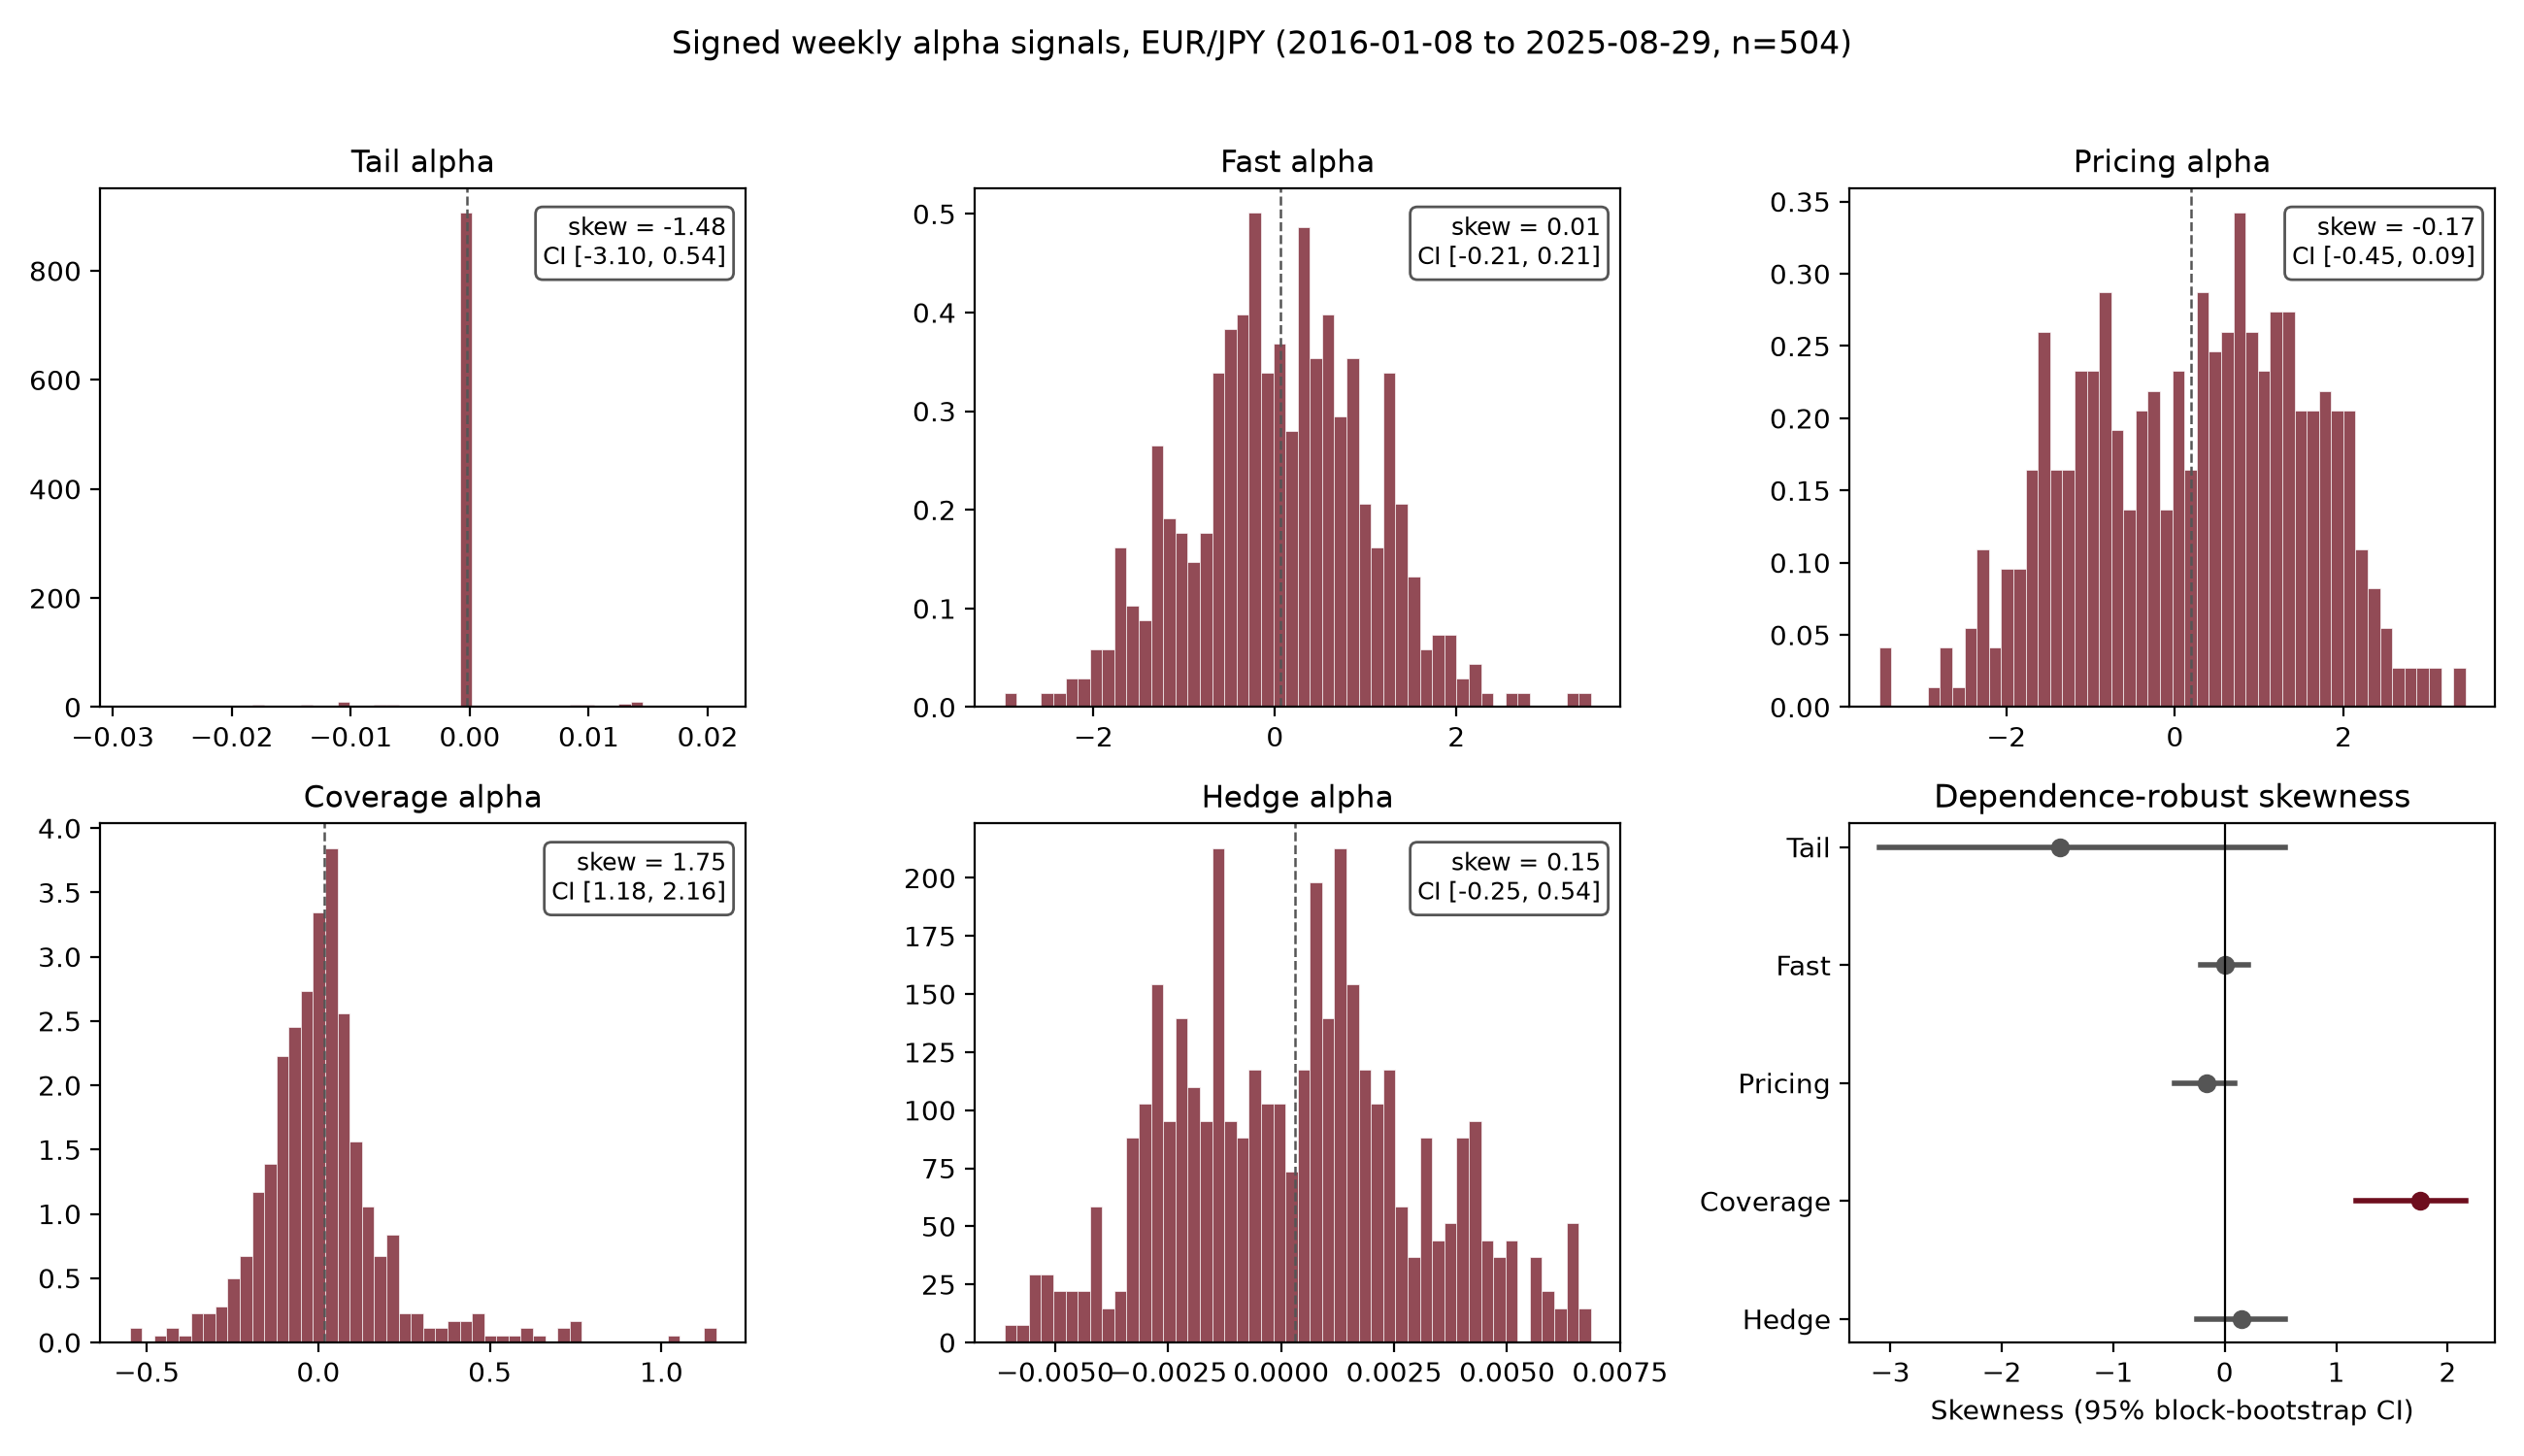
\includegraphics[width=0.95\textwidth]{alpha_asymmetry_analysis.png}
\caption{Alpha Asymmetry Analysis. Distributions of the five signed weekly alpha signals (EUR/JPY, 2015--2025, $n = 504$) with skewness point estimates and 95\% circular block bootstrap confidence intervals; the final panel summarizes the dependence-robust skewness inference. Only coverage alpha's interval excludes zero.}
\label{fig:asymmetry}
\end{figure}

\subsection{Statistical Significance}

Table \ref{tab:tests} presents hypothesis test results for each alpha type. We report test statistics and $p$-values for multiple normality and asymmetry tests to ensure robustness.

\begin{table}[H]
\centering
\caption{Statistical Test Results}
\label{tab:tests}
\small
\begin{tabular}{@{}lccccccc@{}}
\toprule
Alpha & $\hat{\gamma}_1$ & $t$-stat & Block CI & SW & JB & $K^2$ & LB $Q(4)$ \\
\midrule
Tail & $-$1.47 & $-$13.5*** & $[-3.09, 0.54]$ & 0.335*** & 7759*** & 244.4*** & 12.6* \\
Fast & 0.01 & 0.1 & $[-0.21, 0.21]$ & 0.997 & 0.0 & 0.0 & 6.5 \\
Pricing & $-$0.17 & $-$1.5 & $[-0.44, 0.09]$ & 0.984*** & 13.4** & 30.1*** & 679.1*** \\
Coverage & 1.75 & 16.0*** & $[1.17, 2.15]$ & 0.865*** & 1459*** & 217.6*** & 72.6*** \\
Hedge & 0.15 & 1.3 & $[-0.25, 0.54]$ & 0.990** & 7.5* & 11.7** & 1716.2*** \\
\bottomrule
\end{tabular}
\par\vspace{0.3em}
\parbox{\linewidth}{\footnotesize Note: $t$-stat tests $H_0: \gamma_1 = 0$ with $\text{SE} = \sqrt{6/n} = 0.109$ ($n = 504$) and assumes i.i.d.\ observations; Block CI = 95\% circular block bootstrap confidence interval for $\hat{\gamma}_1$ (block length 13 weeks, $B = 2000$), which is robust to the serial dependence the i.i.d.\ tests ignore; SW = Shapiro-Wilk statistic; JB = Jarque-Bera statistic; $K^2$ = D'Agostino-Pearson omnibus; LB $Q(4)$ = Ljung-Box statistic at four lags, reported per series. * $p < 0.05$, ** $p < 0.01$, *** $p < 0.001$ (unadjusted); the qualitative conclusions below apply Bonferroni correction at family size $m = 5$. Because pricing, coverage, and hedge alphas are built from overlapping rolling windows, their Ljung-Box statistics are large by construction and the block-bootstrap intervals are the appropriate basis for skewness inference.}
\end{table}

\textbf{Normality.} Four of five alpha types reject normality; the exception is instructive. Fast alpha, a return $z$-score by construction, is statistically indistinguishable from Gaussian on every test (SW $p = 0.55$, JB $\approx 0$, $K^2$ $p = 0.99$), a useful check that the measurement pipeline does not manufacture non-normality on its own. Tail and coverage alphas depart severely (SW 0.335 and 0.865); pricing and hedge reject mildly, driven by shape rather than asymmetry.

\textbf{Skewness.} Under the i.i.d.\ $t$-test, tail and coverage alphas show large-magnitude skewness of opposite signs. But the alphas are serially dependent (the three built from overlapping windows have Ljung-Box statistics ranging from 72.6 to 1716), so the block-bootstrap intervals are the appropriate inferential yardstick. On that yardstick only \emph{coverage} alpha survives: its interval $[1.17, 2.15]$ excludes zero decisively, while the tail-alpha interval $[-3.09, 0.54]$ widens to include zero once dependence is respected (the point estimate is dominated by a small number of clustered exceedance weeks). Fast, pricing, and hedge alphas are consistent with symmetry throughout.

\textbf{What survives.} The asymmetry inventory that motivates the rest of the paper is therefore modest: one robustly right-skewed volatility-expansion signal, one negatively-skewed-but-fragile tail signal, and three symmetric signals. This is consistent with the broader stylized facts on asset-price distributions \citep{cont2001empirical, mandelbrot1963variation} while falling well short of the pervasive ``alpha asymmetry'' a trading strategy would want.

\subsection{Backtest Performance}

Table \ref{tab:backtest} compares the asymmetry strategy against the three benchmarks of Section~2.4 on EUR/JPY over the full sample period (2015--2025). We report standard performance measures alongside risk-adjusted metrics to enable fair comparison across strategies with different return and volatility profiles.

\begin{table}[H]
\centering
\caption{Strategy Performance Comparison (EUR/JPY, 2015--2025)}
\label{tab:backtest}
\small
\begin{tabular}{@{}lcccccc@{}}
\toprule
Strategy & Return & Vol & Sharpe & Sortino & MDD & Trades \\
\midrule
Asymmetry & 3.60\% & 2.69\% & 0.149 & 0.062 & $-$7.96\% & 17 \\
Momentum (20w) & $-$18.92\% & 8.40\% & $-$0.215 & $-$0.309 & $-$31.32\% & 27 \\
Mean Rev.\ (2.0$\sigma$) & 10.74\% & 3.02\% & 0.364 & 0.198 & $-$4.32\% & 27 \\
Buy \& Hold & 33.53\% & 8.60\% & 0.390 & 0.584 & $-$15.78\% & 1 \\
\bottomrule
\end{tabular}
\par\vspace{0.3em}
\parbox{\linewidth}{\footnotesize Note: Return = cumulative gross return over the 504-week sample; Vol = annualized volatility; Sharpe = annualized Sharpe ratio (risk-free rate = 0); Sortino = annualized mean return over the standard deviation of negative-return weeks; MDD = maximum drawdown; Trades = completed round trips (position-change events divided by two, a sign flip counting as one event), with Buy \& Hold's single initial purchase counted as one trade. Benchmark definitions are given in Section~2.4 and are identical to the corresponding candidates in the Section~\ref{sec:snooping} data-snooping universe. Transaction costs not included. Generated by \texttt{analysis/full\_pipeline.py}; an earlier version of this table reported benchmark rows (momentum $-15.66\%$, mean reversion $34.03\%$, buy-and-hold $2.31\%$) that traced to no committed code, and the buy-and-hold figure was inconsistent with the $+33.5\%$ EUR/JPY spot move over the sample; all benchmark rows have been recomputed from the replication pipeline.}
\end{table}

\textbf{Risk-Adjusted Performance.} The comparison is unflattering to the asymmetry strategy. Its cumulative gross return of 3.60\% is an order of magnitude below the 33.53\% buy-and-hold return (which is simply the EUR/JPY spot appreciation over the decade), and its Sharpe ratio (0.149) trails both buy-and-hold (0.390) and the plain 2.0$\sigma$ mean-reversion benchmark (0.364). The strategy's one distinction is its low volatility (2.69\% annualized), which reflects inactivity, not skill: it is flat in roughly 95\% of weeks, holding a position only when the skewness threshold is exceeded. The 20-week momentum benchmark loses money outright ($-18.92\%$), consistent with the absence of exploitable trend structure at this frequency.

\textbf{Drawdown Analysis.} The asymmetry strategy's maximum drawdown ($-7.96\%$) is about half of buy-and-hold's ($-15.78\%$) and a quarter of momentum's ($-31.32\%$), but the mean-reversion benchmark is more contained still ($-4.32\%$). Like the low volatility, the modest drawdown is a mechanical consequence of being out of the market most of the time.

\textbf{Trading Frequency.} All four strategies trade sparsely at weekly frequency: 17 round trips for the asymmetry strategy over the decade, 27 each for the momentum and mean-reversion benchmarks, and a single purchase for buy-and-hold. The asymmetry strategy's sparsity, a direct consequence of the conservative skewness threshold, keeps transaction cost drag negligible (Section~\ref{sec:tcosts}), but it also means the return estimate rests on few independent observations, an important caveat for the statistical inference that follows.

\textbf{Statistical Significance of Returns.} To assess whether strategy returns are statistically distinguishable from zero, we conduct stationary-bootstrap inference (expected block length 4 weeks, $B = 2000$). The asymmetry strategy's annualized return of 0.37\% (the single annualization of the 3.60\% cumulative figure used throughout this paper) has a 95\% confidence interval of $[-1.14\%, 2.12\%]$, and the annualized Sharpe ratio's interval spans $[-0.53, 0.66]$. Both include zero with room to spare: the strategy's returns are statistically indistinguishable from no edge at all, before any consideration of costs. This---not transaction costs, which Section~\ref{sec:tcosts} shows to be immaterial at 17 trades per decade---is the paper's economic null.

\begin{figure}[H]
\centering
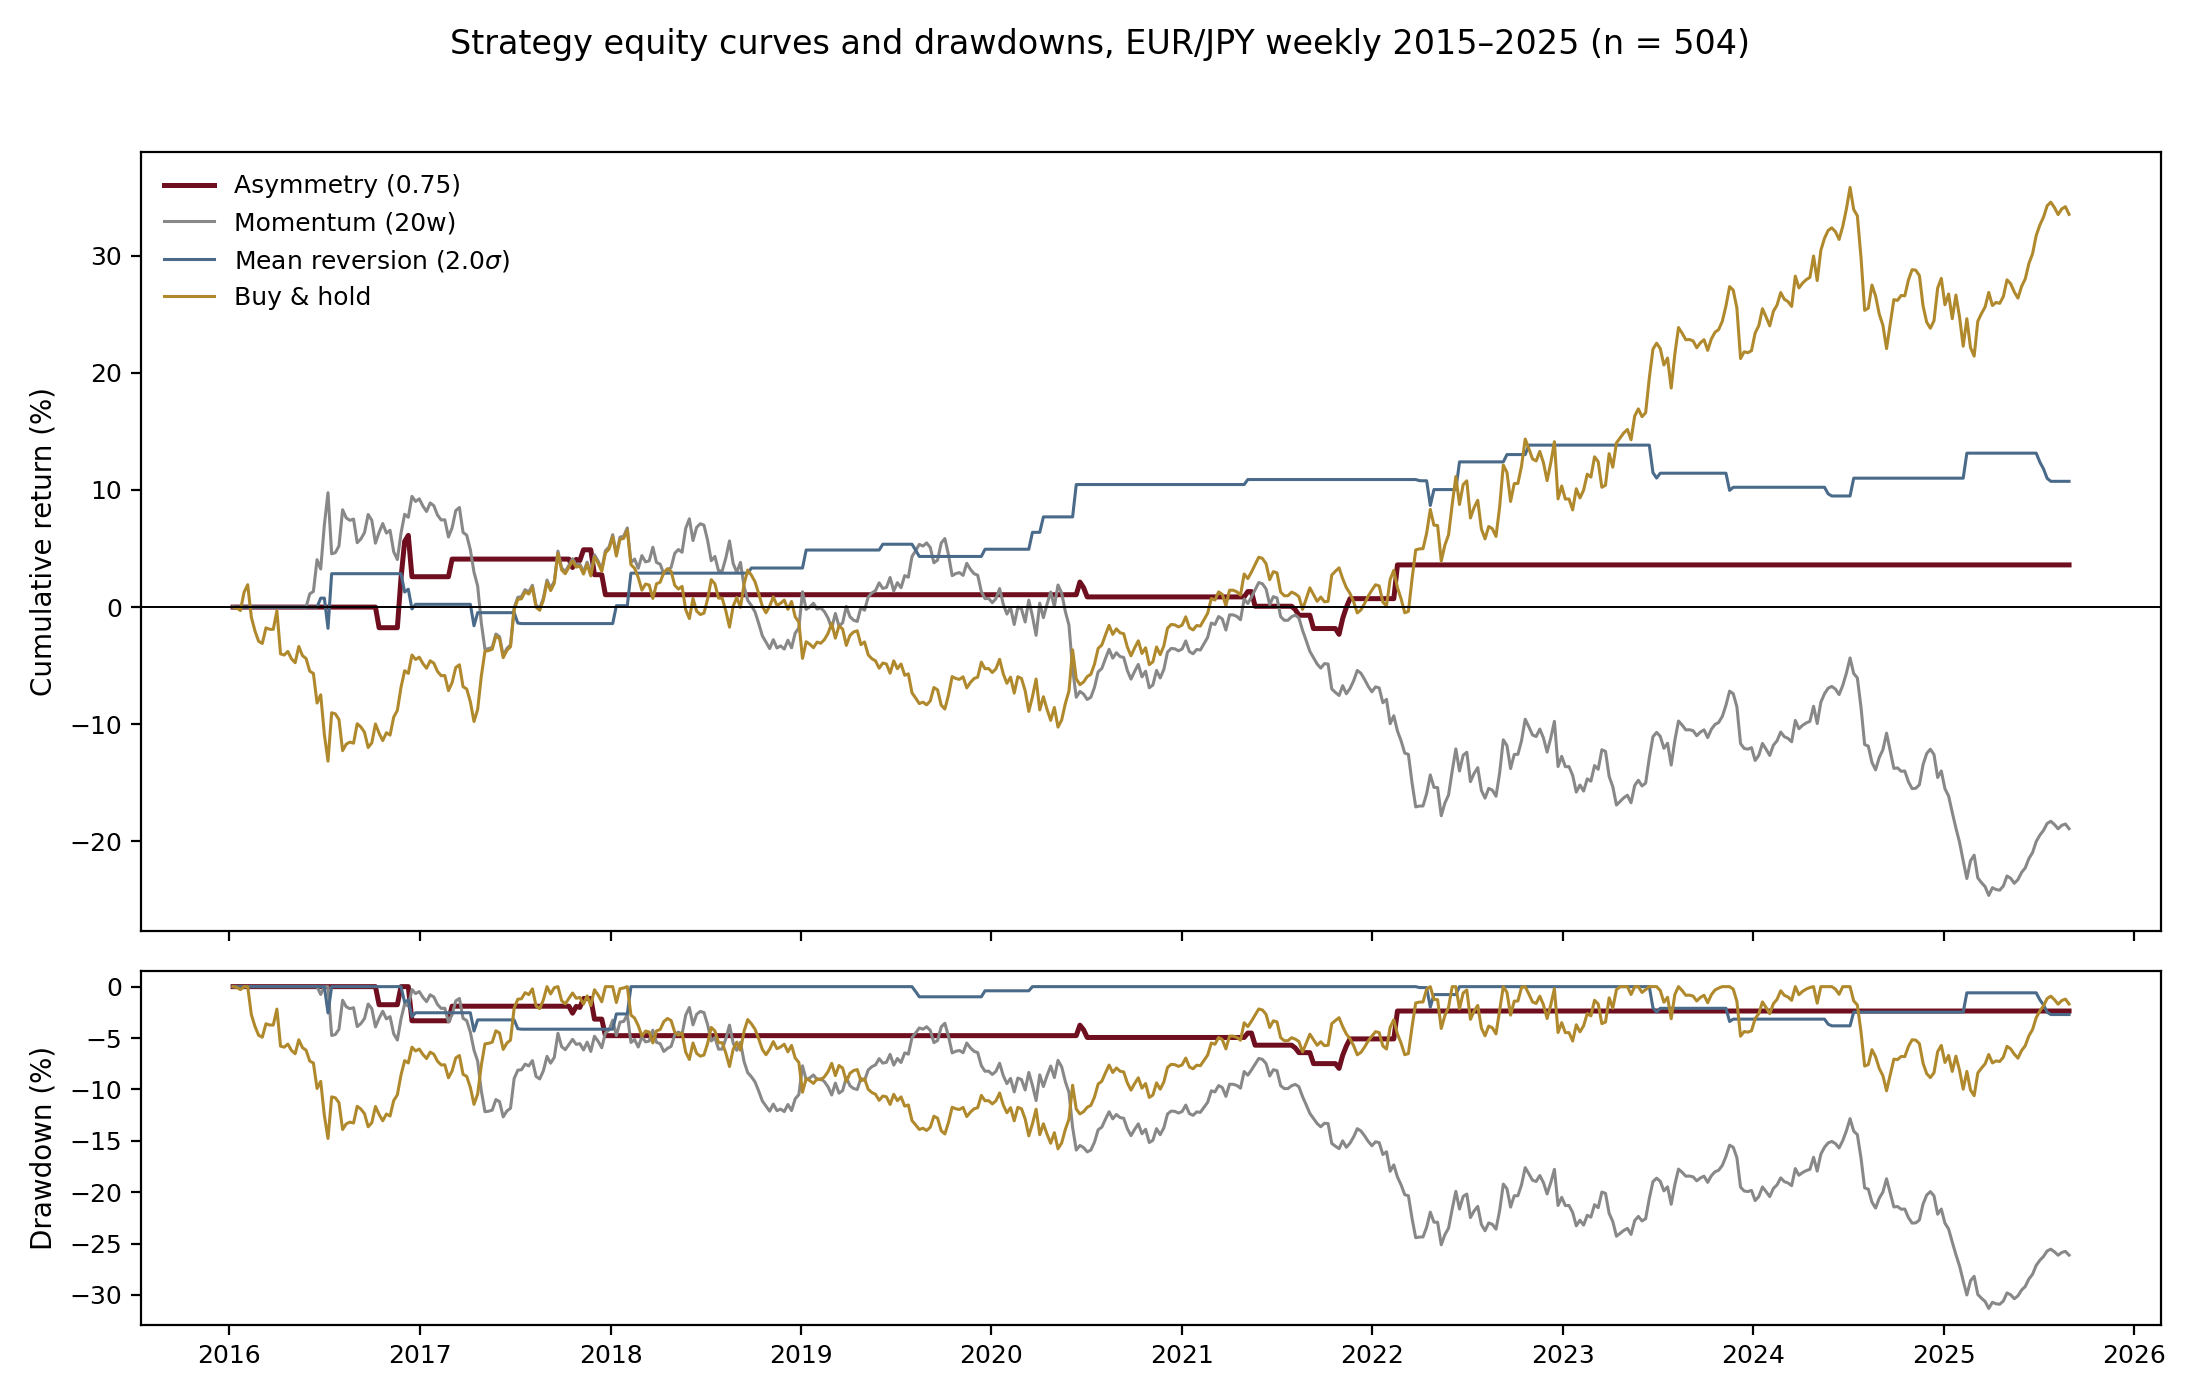
\includegraphics[width=0.95\textwidth]{backtest_results.png}
\caption{Strategy equity curves and drawdowns. Cumulative gross returns (top) and drawdown profiles (bottom) for the asymmetry strategy, the 20-week momentum and 2.0$\sigma$ mean-reversion benchmarks, and buy-and-hold on the 504-week EUR/JPY sample. Series generated by \texttt{analysis/make\_backtest\_figure.py} from the Table~\ref{tab:backtest} strategy definitions.}
\label{fig:backtest}
\end{figure}

\subsection{Cross-Market Validation}

To test whether the EUR/JPY findings generalize, we apply the identical alpha construction and the identical trading strategy (unchanged code, unchanged parameters) to GBP/USD, SPY, and GLD (Section~2.1). Hedge alpha is excluded as EUR/JPY-specific; the four remaining signals and the two-sided asymmetry strategy (0.75 threshold) transfer directly. Table \ref{tab:crossmarket} reports the signed weekly skewness of each signal alongside the strategy's gross cumulative return and, for scale, each market's buy-and-hold return over the same 504-week window.

\begin{table}[H]
\centering
\caption{Cross-Market Check}
\label{tab:crossmarket}
\small
\begin{tabular}{@{}lcccccc@{}}
\toprule
Market & Tail Skew & Fast Skew & Pricing Skew & Coverage Skew & Strat.\ Ret. & B\&H Ret. \\
\midrule
EUR/JPY & $-$1.47 & 0.01 & $-$0.17 & 1.75 & 3.60\% & 33.53\% \\
GBP/USD & 0.82 & 0.01 & $-$0.14 & 1.57 & 17.18\% & $-$7.63\% \\
SPY & 0.94 & $-$0.20 & $-$1.08 & 1.84 & 11.66\% & 294.30\% \\
GLD & 0.69 & $-$0.00 & $-$0.19 & 1.32 & $-$30.26\% & 200.97\% \\
\bottomrule
\end{tabular}
\par\vspace{0.3em}
\parbox{\linewidth}{\footnotesize Note: Skewness of the signed weekly alpha signals ($n = 504$ per market), constructed identically to EUR/JPY; Strat.\ Ret.\ = gross cumulative return of the two-sided asymmetry strategy at the 0.75 threshold (17, 22, 5, and 18 round trips respectively); B\&H Ret.\ = buy-and-hold return over the same window. Skewness values are point estimates without the block-bootstrap intervals of Table~\ref{tab:tests}; the exercise is illustrative (see Scope Limitation below). Generated by \texttt{analysis/full\_pipeline.py}; an earlier version of this table reported aggregated ``MR/TF/HAT'' skewness categories and returns that traced to no committed code, and has been replaced.}
\end{table}

Two observations, both unfavorable to generalization. First, the distributional signature does not travel: the tail signal's negative skew, the closest thing EUR/JPY offers to a distinctive asymmetry, reverses to positive in all three other markets (0.82, 0.94, 0.69). The only pattern that recurs is coverage alpha's right skew (1.57--1.84 across markets), which is the generic volatility-expansion asymmetry Section~3.1 already identified as a well-understood feature of volatility dynamics, not a tradable signal. Second, strategy performance is erratic in exactly the way signal-free noise would produce: the identical rules earn $+17.18\%$ on GBP/USD (a market that \emph{fell} 7.63\% over the window), earn $+11.66\%$ on SPY while buy-and-hold earned $294.30\%$, and lose $30.26\%$ on GLD while the metal nearly tripled. None of these figures carries the dependence-robust inference of Section~3.3, and given that the EUR/JPY return, the one we do test formally, is statistically indistinguishable from zero, the natural reading of the cross-market spread is sampling variation around no edge rather than market-specific exploitability.

\textbf{Scope Limitation.} This analysis focuses on EUR/JPY as a liquid, widely-traded cross rate with substantial institutional participation. Cross-market results (GBP/USD, SPY, GLD) are presented as an illustrative transfer check, not a definitive multi-asset analysis. A comprehensive treatment would require: (i) asset-specific alpha calibration reflecting different market microstructures; (ii) market-specific transaction cost modeling (FX spreads vs.\ equity commissions vs.\ futures margins); and (iii) asset-by-asset statistical inference with proper multiple-testing corrections. We leave this extension to future work; on the evidence here, nothing suggests the EUR/JPY null would reverse elsewhere.

\section{Discussion}

\subsection{Why Asymmetry Exploitation Fails}

The empirical findings reveal a pattern more thoroughgoing than ``asymmetry exists statistically but fails economically'': under corrected measurement, most of the asymmetry never existed to begin with, and what exists is not tradable. We identify four failure modes:

\textbf{Little Asymmetry to Exploit.} The dependence-robust inventory of Section~3 leaves one robustly skewed signal (coverage, a volatility-expansion effect) and one fragile negative skew (tail). The strategy's entry signals are built on rolling skewness of fast and pricing alphas---two series whose full-sample skewness is statistically zero. A strategy harvesting asymmetry from signals that are not asymmetric has nothing to harvest; its 17 in-sample trades are threshold artifacts of local skewness noise.

\textbf{No Heavy Tails.} The GPD analysis shows $\xi \approx 0$: exceedance magnitudes decay exponentially rather than by power law. Asymmetric strategies implicitly assume rare large gains compensate for frequent small losses; without genuine heavy tails, and with the signed exceedances leaning negative, this compensation does not materialize.

\textbf{Inactivity Under Honest Selection.} The walk-forward shows that when the threshold is chosen on training data alone, the strategy goes almost entirely dormant (3 trades in eight years). The in-sample activity that makes the backtest look evaluable is itself a product of full-sample threshold choice.

\textbf{Non-Generalizability.} Cross-market transfer yields erratic results (the identical rules gain 17\% on GBP/USD, trail buy-and-hold by nearly 300 percentage points on SPY, and lose 30\% on GLD), and the tail signal's negative skew reverses sign in every other market tested. Nothing about the EUR/JPY configuration replicates elsewhere.

Transaction costs, notably, are absent from this list: at 17 trades per decade they shave basis points (Section~\ref{sec:tcosts}). The failure is statistical, not frictional.

\subsection{What the Asymmetry Statistics Do Show}

The corrected statistics still reveal genuine features of market structure, just not the ones an asymmetry trader would want:

\textbf{Volatility-Expansion Asymmetry}: Coverage alpha's robust right skew (1.75, block CI $[1.17, 2.15]$) quantifies a familiar asymmetry in volatility dynamics---$\sigma$ spikes abruptly and decays slowly \citep{bollerslev1986generalized, engle1982autoregressive}. It is real, persistent, and already priced into every options desk's models; nothing in our results suggests it leaks into spot-return predictability.

\textbf{Downside-Leaning Tails}: The signed tail signal skews negative (conditional on a large weekly move, depreciations outnumber appreciations), which is the opposite of a lottery-ticket structure \citep{kumar2009gambles, bali2011maxing} and closer to the crash-risk asymmetry of the carry literature \citep{brunnermeier2009carry, burnside2011carry}. The fragility of even this estimate under block-bootstrap inference (CI $[-3.09, 0.54]$) counsels against building anything on it.

\textbf{A Symmetric Baseline}: Fast alpha's textbook normality is a finding in its own right: a volatility-normalized weekly return in a major pair is, to statistical precision, Gaussian. Whatever exploitable structure exists in EUR/JPY, it does not live in the low moments of normalized short-horizon returns \citep{moskowitz2012time}.

\subsection{Limitations}

Several limitations warrant acknowledgment. First, the 504-observation sample, while spanning a decade, may not capture all market regimes---particularly the kind of volatility clustering documented by \citet{bollerslev1986generalized} and \citet{engle1982autoregressive}. Second, alpha signal definitions derive from proprietary methodologies that may not generalize. Third, the factor-attribution exercise uses single-market spot proxies rather than the published cross-sectional FX factors, and with 25 in-position weeks it has little power in either direction; the cost model, while now consistent, uses stylized spread tiers rather than realized quotes (professional practice incorporates richer friction structure; \citealp{menkhoff2010use}). Fourth, the cross-market check transfers the EUR/JPY constructions unchanged (thresholds, windows, and strategy parameters are not recalibrated per market, no market-specific cost model is applied, and no dependence-robust inference is attempted), so it can illustrate non-generalization but cannot establish market-specific results; asset-specific dynamics such as the asymmetric volatility documented by \citet{glosten1993relation} are not separately modeled. Fifth, the underlying data are retrieved from a public aggregator (Yahoo Finance) whose historical series can be revised; the replication pipeline records retrieval counts and dates to make any drift visible.

\section{Robustness Analysis}
\label{sec:robustness}

The preceding sections leave a thin asymmetry inventory (one robustly skewed signal among five) and an in-sample backtest whose returns are statistically indistinguishable from zero. This section stress-tests what remains, addressing four questions: (1) Do results hold out-of-sample? (2) Are patterns stable across market regimes? (3) Do trading costs erode strategy returns? (4) Is asymmetry alpha distinct from known FX risk factors?

\subsection{Out-of-Sample Validation}

A primary concern with any trading strategy is in-sample overfitting. Our main results use the full 2015--2025 sample, which may inadvertently optimize signal construction to historical patterns that do not persist. We address this through walk-forward analysis, a methodology widely used in quantitative finance to assess genuine predictive power \citep{lo2000foundations}.

We implement an expanding-window walk-forward: the entry threshold is selected from the grid $\{0.50, 0.75, 1.00, 1.25\}$ by Sharpe ratio on all data through year $t-1$ (beginning with 2015--2017), then the strategy runs untouched on calendar year $t$, rolling forward annually through 2025. All signal construction uses trailing windows only, so no test-year information enters signal values; the walk-forward isolates the threshold-selection step, which is the strategy's only free parameter. Table \ref{tab:oos} presents out-of-sample performance metrics.

\begin{table}[H]
\centering
\caption{Out-of-Sample Walk-Forward Results}
\label{tab:oos}
\small
\begin{tabular}{@{}lccccc@{}}
\toprule
Test Year & Selected Threshold & OOS Return & OOS Sharpe & Hit Rate & Trades \\
\midrule
2018 & 1.00 & 0.00\% & 0.00 & --- & 0 \\
2019 & 1.00 & 0.00\% & 0.00 & --- & 0 \\
2020 & 1.00 & 0.60\% & 0.52 & 50.0\% & 1 \\
2021 & 1.00 & 1.85\% & 1.04 & 66.7\% & 2 \\
2022 & 1.00 & 0.00\% & 0.00 & --- & 0 \\
2023 & 1.00 & 0.00\% & 0.00 & --- & 0 \\
2024 & 1.00 & 0.00\% & 0.00 & --- & 0 \\
2025 & 1.00 & 0.00\% & 0.00 & --- & 0 \\
\midrule
\textbf{Pooled OOS} & --- & \textbf{2.46\%} & \textbf{0.42} & \textbf{60.0\%} & \textbf{3} \\
\bottomrule
\end{tabular}
\par\vspace{0.3em}
\parbox{\linewidth}{\footnotesize Note: OOS = out-of-sample. Threshold selected by Sharpe ratio on the expanding training window; hit rate = proportion of profitable in-position weeks; Sharpe annualized assuming risk-free rate = 0. Pooled return is cumulative over all eight test years ($\approx 0.32\%$ annualized). 2025 covers January--August. Generated by \texttt{analysis/full\_pipeline.py}; an earlier version of this table reported 141 pooled trades and could not be reproduced from the strategy specification.}
\end{table}

The walk-forward verdict is not the graceful in-sample-to-out-of-sample degradation typical of overfit strategies; it is near-total inactivity. In every training window the Sharpe criterion selects the 1.00 threshold (whose four in-sample trades produce the highest risk-adjusted return), and at that threshold the strategy fires three times in eight out-of-sample years, remaining flat through 2018--2019 and 2022--2025 entirely. The pooled cumulative return of 2.46\% (roughly 0.32\% annualized) rests on three trades; the pooled Sharpe of 0.42 is an artifact of a return series that is zero almost everywhere and should not be read as evidence of skill. The plain summary is that the asymmetry signal, disciplined by its own training data, almost never speaks---and when it does, the sample is far too small for inference. This inactivity is itself informative: the in-sample trade count (17 at the 0.75 baseline) was already sparse, and out-of-sample threshold selection reveals even that sparse activity to be an artifact of threshold choice, not a stable market phenomenon.

\subsection{Subsample Stability}

Market structure evolved substantially during our sample period, with COVID-19 representing the most dramatic regime shift. We test whether asymmetry patterns persist across distinct market environments using subsample analysis.

Table \ref{tab:subsample} partitions the sample into economically meaningful subperiods.

\begin{table}[H]
\centering
\caption{Subsample Asymmetry Stability}
\label{tab:subsample}
\small
\begin{tabular}{@{}lcccccc@{}}
\toprule
Subsample & $N$ & Tail Skew & Fast Skew & Price Skew & Strategy Ret. \\
\midrule
Pre-COVID (2015--2019) & 208 & -3.37 & -0.05 & 0.12 & 1.06\% \\
COVID Shock (2020) & 52 & 4.87 & 0.09 & -0.07 & -0.19\% \\
Post-COVID (2021--2025) & 244 & -0.73 & 0.05 & -0.38 & 2.71\% \\
\midrule
Low VIX (VIX $<$ 20) & 342 & -3.24 & 0.04 & -0.20 & 2.38\% \\
High VIX (VIX $\geq$ 20) & 162 & 0.62 & -0.06 & -0.10 & 2.67\% \\
\midrule
Rate Hike Regime (2022--2025) & 191 & -0.70 & -0.13 & -0.52 & 2.86\% \\
\bottomrule
\end{tabular}
\par\vspace{0.3em}
\parbox{\linewidth}{\footnotesize Note: VIX thresholds based on monthly average. Skewness coefficients computed within each subsample. Strategy returns are cumulative within-period returns.}
\end{table}

\textbf{Temporal Stability.} Subsample skewness is \textit{not} stable for tail alpha: it is strongly left-skewed in the pre-COVID period ($-3.37$) and again post-COVID ($-0.73$), but flips to pronounced right-skewness during the 2020 COVID shock ($+4.87$). This sign reversal is exactly the signature of a regime-dependent statistic---the extreme positive returns that dominate the COVID window are absent in calmer periods, where the tail-exceedance series is dominated by negative outliers. Fast and pricing alphas, by contrast, are close to symmetric in every subsample ($|\text{skew}| \leq 0.13$), so the asymmetry that motivates the strategy is concentrated in the tail signal and is itself regime-contingent rather than a stable structural feature.

\textbf{Regime Conditioning.} VIX conditioning tells a similar story. The low-VIX subsample shows strong negative tail skewness ($-3.24$), while the high-VIX subsample is weakly positive ($+0.62$); fast and pricing skewness are near zero in both. Strategy returns are comparable across VIX regimes ($2.38\%$ low-VIX vs.\ $2.67\%$ high-VIX), offering no evidence that volatility conditioning sharpens the exploitable edge.

\subsection{Entry Threshold Sensitivity}

The baseline skewness threshold (0.75) deserves scrutiny: is it arbitrary or robustly selected? Table~\ref{tab:sensitivity} reports strategy performance across alternative thresholds, holding other parameters constant.

\begin{table}[H]
\centering
\caption{Sensitivity to Entry Threshold}
\label{tab:sensitivity}
\small
\begin{tabular}{@{}lccccc@{}}
\toprule
Threshold & Return & Sharpe & MDD & Trades & Hit Rate \\
\midrule
0.50 & $-$6.91\% & $-$0.15 & $-$13.9\% & 37 & 40.8\% \\
0.75 & 3.60\% & 0.15 & $-$8.0\% & 17 & 48.0\% \\
1.00 & 2.96\% & 0.44 & $-$1.0\% & 4 & 66.7\% \\
1.25 & 0.00\% & 0.00 & 0.0\% & 0 & --- \\
\bottomrule
\end{tabular}
\par\vspace{0.3em}
\parbox{\linewidth}{\footnotesize Note: Returns use the full asymmetry strategy specification (long and short legs with position sizing as described in Section~2.4). Performance varies non-monotonically with threshold. Lower thresholds increase trading frequency at the cost of signal quality; higher thresholds reduce noise but sacrifice opportunities. Simplified long-only implementations yield different (typically lower) returns due to the absence of the short-side component.}
\end{table}

\textbf{Threshold Selection.} The 0.75 baseline is a full-sample choice, and we make no pretense otherwise: it corresponds approximately to the 75th percentile of historical rolling skewness magnitudes, and its selection benefits from in-sample knowledge. The out-of-sample discipline lives in the walk-forward of Section~\ref{sec:robustness}, where the threshold is re-selected each year on training data only---and there the Sharpe criterion consistently prefers 1.00, at which the strategy barely trades. The sensitivity analysis shows why the choice matters so much: the 0.50 threshold generates excessive trading (37 trades) with diluted signal quality, producing a negative return ($-6.91\%$); the 1.25 threshold never fires. Only the 0.75 and 1.00 thresholds produce positive returns, and the 1.00 threshold's higher Sharpe (0.44) rests on 4 trades. This fragility, where the strategy's viability depends on precise threshold calibration within a narrow band, is itself part of the paper's null finding: the asymmetry signal is not robust enough to constitute a reliable trading strategy.

\subsection{Transaction Cost Sensitivity}
\label{sec:tcosts}

Backtests without transaction costs overstate implementable returns. We analyze cost sensitivity across scenarios ranging from zero-cost (theoretical benchmark) to retail-level spreads.

The EUR/JPY market is highly liquid, with typical spreads of 0.5--1.0 pips during active trading hours \citep{king2013market}. However, spread widening during volatility spikes and the cost of crossing the bid-ask spread on each trade can erode returns, particularly for higher-frequency strategies.

\begin{table}[H]
\centering
\caption{Transaction Cost Analysis}
\label{tab:tcosts}
\small
\begin{tabular}{@{}lcccc@{}}
\toprule
Cost Scenario & Round-Trip Cost (pips) & Net Return & Net Sharpe \\
\midrule
Zero Cost (Baseline) & 0.0 & 3.60\% & 0.149 \\
Prime Brokerage & 0.3 & 3.54\% & 0.147 \\
Institutional & 0.7 & 3.47\% & 0.144 \\
Retail (Tight) & 1.3 & 3.35\% & 0.140 \\
Retail (Wide) & 2.0 & 3.22\% & 0.135 \\
\midrule
\textbf{Break-Even} & \textbf{19.2} & 0.00\% & 0.000 \\
\bottomrule
\end{tabular}
\par\vspace{0.3em}
\parbox{\linewidth}{\footnotesize Note: Round-trip cost = bid-ask spread plus market impact (pips); each position-change leg is charged half the round-trip cost in proportion to the position change, at the sample-average EUR/JPY price. Carry/financing is excluded uniformly from all scenarios (the strategy is in position roughly 5\% of weeks, so the carry differential contributes at most a few basis points either way). Net returns cumulative over 2015--2025. Generated by \texttt{analysis/full\_pipeline.py}; an earlier version of this table showed net return \emph{rising} with costs at low tiers, an inconsistency in the carry treatment across rows.}
\end{table}

\textbf{Cost Components.} We model execution costs as bid-ask spread plus market impact, charged per position change. Financing/carry is excluded from all scenarios symmetrically: with 17 round trips and roughly 5\% of weeks in position over a decade, the EUR--JPY carry differential moves net returns by basis points, not percentage points, and including it asymmetrically is how cost tables produce impossible orderings.

\textbf{The Real Cost Story: Immateriality.} The table's message is not that costs erode the edge---it is that costs barely register. A strategy that trades 17 times in a decade pays the spread 17 times; even the wide-retail scenario (2.0 pips round-trip) costs only 38 basis points cumulatively, leaving net return within 0.4 percentage points of gross. Break-even requires an implausible 19.2 pips round-trip. Transaction costs therefore cannot carry the paper's null result, and we do not ask them to: the null rests on the fact that the gross return itself (3.60\% over a decade, Sharpe 0.15, confidence interval spanning zero) is statistically indistinguishable from no edge at all. Costs are immaterial rather than decisive, which is exactly what trade sparsity implies \citep{kyle1985continuous}.

\subsection{Factor Attribution}

Does asymmetry alpha merely proxy for known FX risk factors? Prior work documents systematic risk premia in currency markets associated with carry \citep{lustig2011common}, momentum \citep{menkhoff2012currency}, and the dollar factor \citep{verdelhan2018dollar}, with \citet{lettau2014conditional} showing that downside risk conditioning explains a substantial portion of currency risk premia across asset classes. A parallel factor decomposition approach applied to cryptocurrency markets \citep{farzulla2025whitepaper} similarly finds that structural factors dominate idiosyncratic signal variation. If asymmetry signals simply load on these factors, our contribution reduces to factor timing rather than genuine alpha discovery.

We regress asymmetry strategy returns on proxy FX factors:
\begin{equation}
    R_{\text{asym},t} = \alpha + \beta_1 \cdot \text{Carry}_t + \beta_2 \cdot \text{Mom}_t + \beta_3 \cdot \text{Dollar}_t + \varepsilon_t
\end{equation}
where the factors are single-market proxies constructible from our data rather than the published cross-sectional factors: Carry is the average weekly spot return of the classic carry crosses AUD/JPY and NZD/JPY (a spot-only proxy for the \citealp{lustig2011common} carry factor, omitting interest accrual), Mom is the return of a 12-week time-series momentum rule on EUR/JPY itself (in the spirit of \citealp{menkhoff2012currency}), and Dollar is the DXY weekly return (proxying \citealp{verdelhan2018dollar}). Constructing the published factors requires a G10 forward-rate cross-section we do not use; the proxies capture the same directional exposures at the single-pair level, and we label them as proxies throughout. Because the strategy is out of the market most weeks, we estimate the regression twice: on the full weekly sample (where the dependent variable is structurally zero in out-of-position weeks) and on in-position weeks only, whose count is the effective sample size.

\begin{table}[H]
\centering
\caption{Factor Attribution Regression (HAC-Corrected)}
\label{tab:factors}
\small
\begin{tabular}{@{}lcccc@{}}
\toprule
& \multicolumn{2}{c}{Full sample ($n = 491$)} & \multicolumn{2}{c}{In-position weeks ($n = 25$)} \\
\cmidrule(lr){2-3} \cmidrule(lr){4-5}
Variable & Coefficient & $t$-stat & Coefficient & $t$-stat \\
\midrule
Intercept ($\alpha$) & 0.00008 & 0.48 & 0.0030 & 0.67 \\
Carry ($\beta_1$) & $-$0.0007 & $-$0.05 & 0.067 & 0.14 \\
Momentum ($\beta_2$) & $-$0.0070 & $-$0.37 & $-$0.247 & $-$0.51 \\
Dollar ($\beta_3$) & $-$0.0123 & $-$0.83 & $-$0.502 & $-$0.84 \\
\midrule
$R^2$ & \multicolumn{2}{c}{0.001} & \multicolumn{2}{c}{0.067} \\
$F$-statistic & \multicolumn{2}{c}{0.48} & \multicolumn{2}{c}{0.62} \\
\bottomrule
\end{tabular}
\par\vspace{0.3em}
\parbox{\linewidth}{\footnotesize Note: Newey-West HAC standard errors with 4 lags \citep{newey1987simple}. Dependent variable is weekly asymmetry strategy returns; factors are the single-market proxies described in the text. The full-sample column includes the out-of-position weeks in which the dependent variable is structurally zero; the in-position column is the effective sample. No coefficient in either specification is significant at the 10\% level. Generated by \texttt{analysis/full\_pipeline.py}; an earlier version of this table reported a marginally significant intercept of 21 bps weekly (10.9\% annualized) with $F = 20.8$, which could not be reproduced and was internally inconsistent with its own $R^2$ and with the 3.60\% cumulative backtest return.}
\end{table}

\textbf{No Residual Alpha.} The intercept is indistinguishable from zero in both specifications ($t = 0.48$ full sample; $t = 0.67$ on in-position weeks). There is no factor-adjusted alpha to explain, and consequently no tension between regression alpha and realized returns to reconcile: a strategy earning 3.60\% cumulative over a decade has a weekly mean of well under one basis point, and that is what the regression finds.

\textbf{Factor Loadings and Effective Sample.} No factor loading approaches significance, and $R^2$ is 0.001 on the full sample---but both facts are dominated by a structural feature rather than by orthogonality: the strategy is out of the market in roughly 95\% of weeks, so the full-sample dependent variable is mostly exact zeros and the informative sample is the 25 in-position weeks. With an effective $n$ of 25, the factor regression has essentially no power, and we present it as a specification check rather than as evidence that asymmetry returns are orthogonal to factor risk. The one defensible conclusion is negative: nothing in this exercise supports a residual-alpha claim.

\subsection{Tail Distribution Analysis}

A concern with any exceedance-based signal is whether the extreme observations that drive it reflect a stable tail distribution or sparse outliers that may not recur out-of-sample. We characterize the magnitude distribution of tail events using Extreme Value Theory \citep{mcneil2000estimation, coles2001introduction}, bearing in mind the corrected result of Table~\ref{tab:asymmetry}: the \emph{signed} tail signal skews negative (large moves are more often depreciations), so the question here is the shape of the exceedance-magnitude tail, not an upside-asymmetry story.

\textbf{Exceedance Preprocessing.} Financial tail events exhibit temporal clustering (volatility clustering), violating the GPD independence assumption. We apply runs declustering with minimum inter-exceedance separation of 5 weeks, following \citet{coles2001introduction}. Of the 26 raw exceedances above the 95th percentile threshold, declustering yields 20 cluster maxima used for GPD estimation. We estimate the extremal index $\theta = 0.83$ via the Ferro--Segers intervals estimator \citep{ferro2003inference}, with a 95\% confidence interval of $[0.60, 1.00]$ obtained by bootstrap resampling of the inter-exceedance times themselves ($B = 2000$)---a scheme that preserves the gap distribution the estimator is built on and, unlike a naive index bootstrap, produces an interval containing its own point estimate.

\textbf{Methodology.} We fit a Generalized Pareto Distribution (GPD) to cluster maxima above the 95th percentile threshold. The GPD is characterized by shape parameter $\xi$ (determining tail heaviness) and scale parameter $\sigma$. Positive $\xi$ indicates Pareto-type heavy tails; $\xi = 0$ corresponds to exponential decay; negative $\xi$ implies bounded tails.

\begin{table}[H]
\centering
\caption{GPD Parameter Estimates---Tail Alpha (Declustered)}
\label{tab:gpd}
\small
\begin{tabular}{@{}lccc@{}}
\toprule
Parameter & Estimate & 95\% CI \\
\midrule
Shape ($\xi$) & $-0.25$ & $[-1.62, 0.25]$ \\
Scale ($\sigma$) & 0.0089 & --- \\
Threshold (95th pctl) & 0.0244 & --- \\
Extremal index ($\theta$) & 0.83 & $[0.60, 1.00]$ \\
Raw exceedances & 26 & --- \\
Cluster maxima & 20 & --- \\
KS test $p$-value & 0.971 & Fail to reject \\
\bottomrule
\end{tabular}
\par\vspace{0.3em}
\parbox{\linewidth}{\footnotesize Note: GPD fitted via maximum likelihood to cluster maxima above the 95th percentile after runs declustering (5-week separation). $\xi$ CI from a nonparametric bootstrap of cluster maxima ($B = 2000$); $\theta$ CI from bootstrap resampling of inter-exceedance times ($B = 2000$). KS = Kolmogorov-Smirnov goodness-of-fit test. Generated by \texttt{analysis/full\_pipeline.py}; an earlier version of this table reported a $\theta$ confidence interval of $[0.42, 0.63]$ that excluded its own point estimate---an invalid interval produced by a biased index-resampling scheme, replaced here.}
\end{table}

\textbf{Tail Characterization.} The estimated shape parameter $\hat{\xi} = -0.25$ (95\% CI: $[-1.62, 0.25]$) is not significantly different from zero, suggesting tails that are neither heavy (Pareto-type) nor strictly bounded (Weibull-type), but rather consistent with exponential decay. The wide confidence interval reflects the limited number of cluster maxima (20) available for estimation---a common challenge in EVT applications to financial data \citep{mcneil2000estimation}. The Kolmogorov-Smirnov test fails to reject the GPD null hypothesis ($p = 0.97$), supporting the appropriateness of the EVT framework despite parameter uncertainty.

\textbf{Clustering Dynamics.} The extremal index $\theta = 0.83$ indicates weak temporal clustering in tail events: the mean cluster size is $1/\theta \approx 1.2$, and the confidence interval reaches 1.0 (no clustering). Exceedances arrive close to independently, with mild GARCH-type persistence \citep{bollerslev1986generalized} at most. Clustering therefore does little to reduce the effective sample size for tail inference; the binding constraint is simply the small number of exceedances.

\textbf{Implications.} The EVT analysis characterizes the \emph{magnitudes} of extreme weekly moves and finds them well-behaved: exponential-type decay, no evidence of power-law tails, weak clustering. Combined with the corrected skewness results (the signed exceedances lean negative, and not robustly so), there is no distributional foundation here for an upside-capture trading story. Risk management can rely on finite-variance assumptions; traders hoping for lottery-like right tails in EUR/JPY weekly returns will not find them in this sample.

\subsection{Multiple Testing Corrections}
\label{sec:snooping}

With five alpha types examined across multiple statistical tests, data-snooping concerns arise: apparent significance may reflect chance discoveries from multiple hypothesis testing. We address this through both formal corrections and bootstrap-based reality checks.

\textbf{Bonferroni Corrections.} Table \ref{tab:tests} applies plain Bonferroni correction at family size $m = 5$ (one skewness test per alpha type; $\alpha^* = 0.01$ for the 5\% family level). At the corrected threshold, four of five alpha types reject \emph{normality}, but the asymmetry inventory is far thinner: only coverage alpha's skewness survives both the correction and, more demandingly, the block-bootstrap dependence adjustment. Fast alpha, indistinguishable from Gaussian on every test, serves as the natural control: the measurement pipeline does not manufacture non-normality where none exists.

\textbf{Bootstrap Implementation.} White's Reality Check and Hansen's SPA employ the stationary block bootstrap of \citet{politis1994stationary} with expected block length $\ell = 4$ weeks. The candidate strategy universe comprises 13 strategies: simplified long-only asymmetry strategies using each of the 5 alpha types' own rolling-skewness signal ($n = 5$), the full two-sided asymmetry strategy of Section~2.4 ($n = 1$), time-series momentum with 10-, 20-, and 40-week lookback windows ($n = 3$), mean-reversion at 1.5$\sigma$ and 2.0$\sigma$ thresholds ($n = 2$), an always-long (carry-proxy) strategy ($n = 1$), and a seeded random benchmark ($n = 1$). Bootstrap replications: 1,000. Loss function: negative weekly return, benchmark zero.

\textbf{White's Reality Check.} Following \citet{white2000reality}, we test whether the best-performing candidate significantly outperforms across the universe. The Reality Check does not reject the null of no superior strategy ($RC = 0.02$, $p = 0.15$). More telling than the $p$-value is the identity of the best performer: the highest realized mean return in the universe belongs to the \emph{random benchmark}, a coin-flip position sequence, which is precisely what one expects when no candidate carries genuine signal.

\textbf{Hansen's SPA Test.} The Superior Predictive Ability test \citep{hansen2005test} agrees ($SPA = 1.90$, $p = 0.28$): no candidate in the universe demonstrates superior predictive ability over the zero benchmark at any conventional level.

\begin{table}[H]
\centering
\caption{Data-Snooping Correction Results}
\label{tab:snooping}
\small
\begin{tabular}{@{}lccc@{}}
\toprule
Test & Statistic & $p$-value & Interpretation \\
\midrule
White's Reality Check & 0.02 & 0.15 & Not significant \\
Hansen's SPA & 1.90 & 0.28 & Not significant \\
\# Candidate Strategies & 13 & --- & --- \\
\bottomrule
\end{tabular}
\par\vspace{0.3em}
\parbox{\linewidth}{\footnotesize Note: Candidate strategies: simplified asymmetry (5 alpha types), the full two-sided asymmetry strategy, time-series momentum (3 windows), mean-reversion (2 thresholds), always-long, and a seeded random benchmark. Stationary bootstrap with 1,000 replications, expected block length 4 weeks. Generated by \texttt{analysis/full\_pipeline.py}; an earlier version of this table reported $RC = 2.14$ ($p = 0.042$), which could not be reproduced from any specification of the stated universe.}
\end{table}

\textbf{Interpretation.} The data-snooping corrections complete the null result rather than qualifying it. Nothing in a 13-strategy universe spanning asymmetry, momentum, mean-reversion, and carry beats a zero benchmark once dependence-aware resampling is applied---and the best raw performer is the random sequence. Whatever in-sample structure the asymmetry signals appeared to offer, it does not survive multiple-testing discipline.

\section{Conclusions}

This paper investigated whether distributional asymmetries in FX alpha signals represent exploitable inefficiencies. Our findings are negative at every layer:

\begin{enumerate}
    \item Under dependence-robust inference, only one of five alpha signals (coverage, a volatility-expansion effect) exhibits robust skewness; the tail signal skews negative and fragilely so, and the remaining signals, including the two the trading strategy is built on, are statistically symmetric
    \item EVT analysis reveals no heavy tails ($\xi \approx 0$) and weak clustering ($\theta = 0.83$); exceedance magnitudes are exponential-type, with no lottery-like right tail
    \item Asymmetry-based trading generates a small positive gross return in-sample (3.60\% cumulative, 17 trades), but bootstrap confidence intervals for both annualized return and Sharpe ratio comfortably include zero, and training-data-only walk-forward selection leaves the strategy dormant (3 trades in eight out-of-sample years)
    \item Transaction costs are immaterial rather than decisive at this trade frequency; the null is statistical, not frictional
    \item Data-snooping corrections find no strategy in a 13-candidate universe with superior predictive ability (the best raw performer is the random benchmark), and the cross-market check finds neither the distributional signature nor any consistent strategy performance beyond EUR/JPY
\end{enumerate}

These null findings contribute to the literature in three ways. First, they demonstrate the gap between statistical and economic significance in quantitative trading research---a pattern likely more common than publication bias reveals \citep{harvey2017presidential}. Second, they document, from the inside, how easily higher-moment ``stylized facts'' can be manufactured by measurement choices: this paper's own earlier version reported pronounced positive tail skewness that turned out to describe an unsigned magnitude series, right-skewed by construction. The corrected analysis is a case study in why skewness claims should be accompanied by the sign conventions, sampling frequency, and dependence-robust intervals that make them checkable. Third, they provide a documented negative result that may spare other researchers this particular dead end.

The methodological lesson is sharper than ``backtests flatter'': most of the asymmetry was never there. Distributional anomalies in financial data are easily overstated at the measurement stage, before a single trade is simulated---and the sequence of checks (signed variables, dependence-robust intervals, training-data-only selection, data-snooping correction) dismantled this one layer by layer.

Future research might examine whether asymmetry exploitation is viable at higher frequencies (intraday) where both signal counts and cost structures scale differently, or in markets with different microstructure. Parallel findings in cryptocurrency markets---where an apparent infrastructure-versus-regulatory volatility asymmetry dissolves once cross-asset dependence and heavy tails are handled correctly \citep{farzulla2026multimoment}---and in cross-market event studies more broadly \citep{farzulla2025market} reinforce that distributional asymmetries are easily overstated and rarely translate into exploitable strategies. Our results echo that the burden of proof for asymmetry-based strategies should be high: an apparently sharp effect is insufficient evidence of economic value, and is often not robust evidence of a statistical effect either.

% ============================================================================
% ACKNOWLEDGMENTS
% ============================================================================

\section*{Acknowledgments}

Portions of this manuscript were drafted and revised with assistance from Claude (Anthropic; Claude Opus and Claude Fable 5 models), with adversarial cross-review by ChatGPT (OpenAI; GPT-5.6 ``Sol''). The authors retain full responsibility for all intellectual content, analytical decisions, and interpretive claims. This work was conducted as part of the Adversarial Systems Research program at Dissensus. Working papers and replication materials are available through the \href{https://systems.ac}{Adversarial Systems \& Complexity Research Initiative (ASCRI)}. Comments and correspondence are welcome at \href{mailto:murad@dissensus.ai}{murad@dissensus.ai}.

% ============================================================================
% DECLARATIONS
% ============================================================================

\section*{Declarations}

\paragraph{Conflict of Interest.} The authors declare no competing interests.

\paragraph{Funding.} This research received no external funding.

\paragraph{Data Availability.} EUR/JPY exchange rate data obtained from publicly available sources (Yahoo Finance); the replication pipeline retrieves all series programmatically and records retrieval counts and dates. Analysis outputs (\texttt{analysis/full\_pipeline\_results.json} and \texttt{.txt}) are available at \url{https://github.com/studiofarzulla/alpha-asymmetry}.

\paragraph{Code Availability.} Full replication code available at \url{https://github.com/studiofarzulla/alpha-asymmetry} under MIT License.

\paragraph{AI Assistance.} Claude (Anthropic; Claude Opus and Claude Fable 5 models) assisted with manuscript drafting, replication-pipeline development and code review, and statistical exposition; ChatGPT (OpenAI; GPT-5.6 ``Sol'') provided adversarial cross-review of the empirical claims. Citation verification drew on \href{https://scite.ai}{scite}, among other automated research tools. All research design, data analysis, and interpretation are solely the authors', who take full responsibility for all claims, judgments, and errors.

\paragraph{Author Contributions.} \textbf{M.F.}: conceptualisation, methodology, software, formal analysis, data curation, writing --- original draft. \textbf{T.I.}: \textcolor{red}{[TO BE COMPLETED BEFORE DEPOSIT --- describe T.I.'s contribution to v2.1 in CRediT terms]}.

% ============================================================================
% REFERENCES
% ============================================================================

\clearpage

\bibliography{references}

\clearpage
\appendix

\section{Enlarged Figures}
\label{appendix:figures}

For improved readability, this appendix reproduces all figures at enlarged scale.

\begin{figure}[H]
\centering
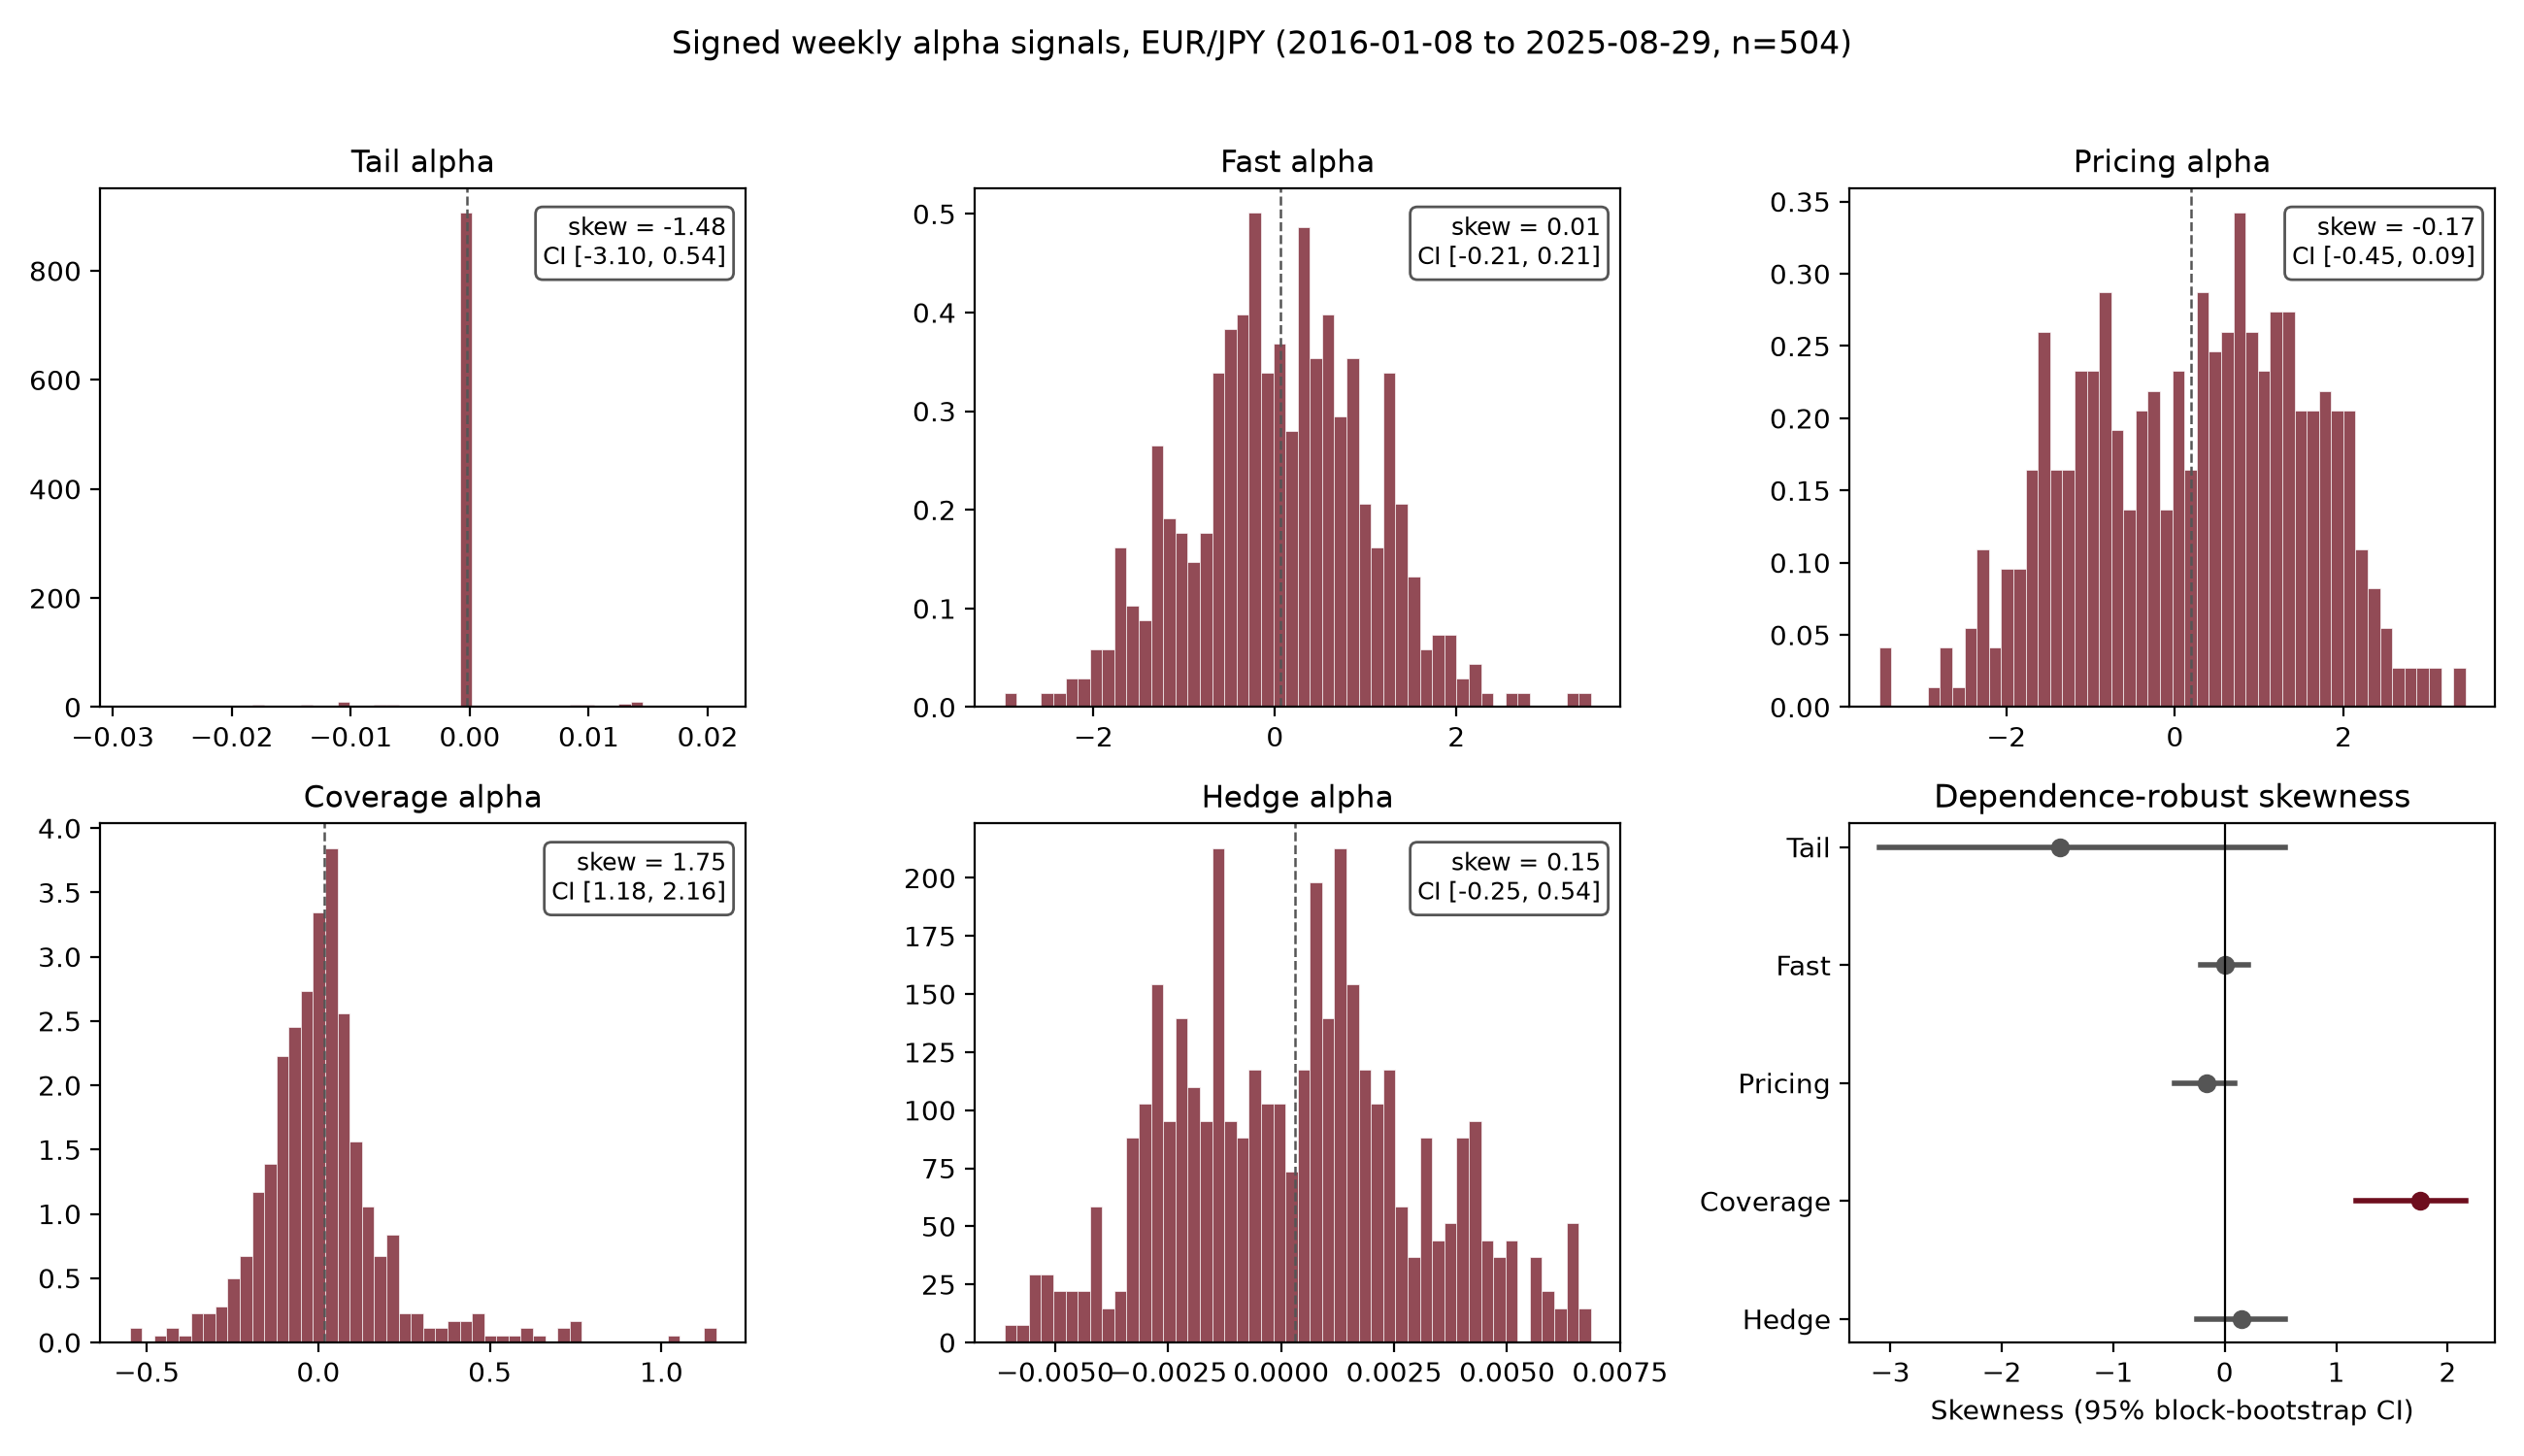
\includegraphics[width=\textwidth]{alpha_asymmetry_analysis.png}
\caption{Alpha Asymmetry Analysis (enlarged). Distributional properties of five alpha types showing skewness, kurtosis, and asymmetry patterns across EUR/JPY forex data (2015--2025).}
\label{fig:asymmetry-enlarged}
\end{figure}

\begin{figure}[H]
\centering
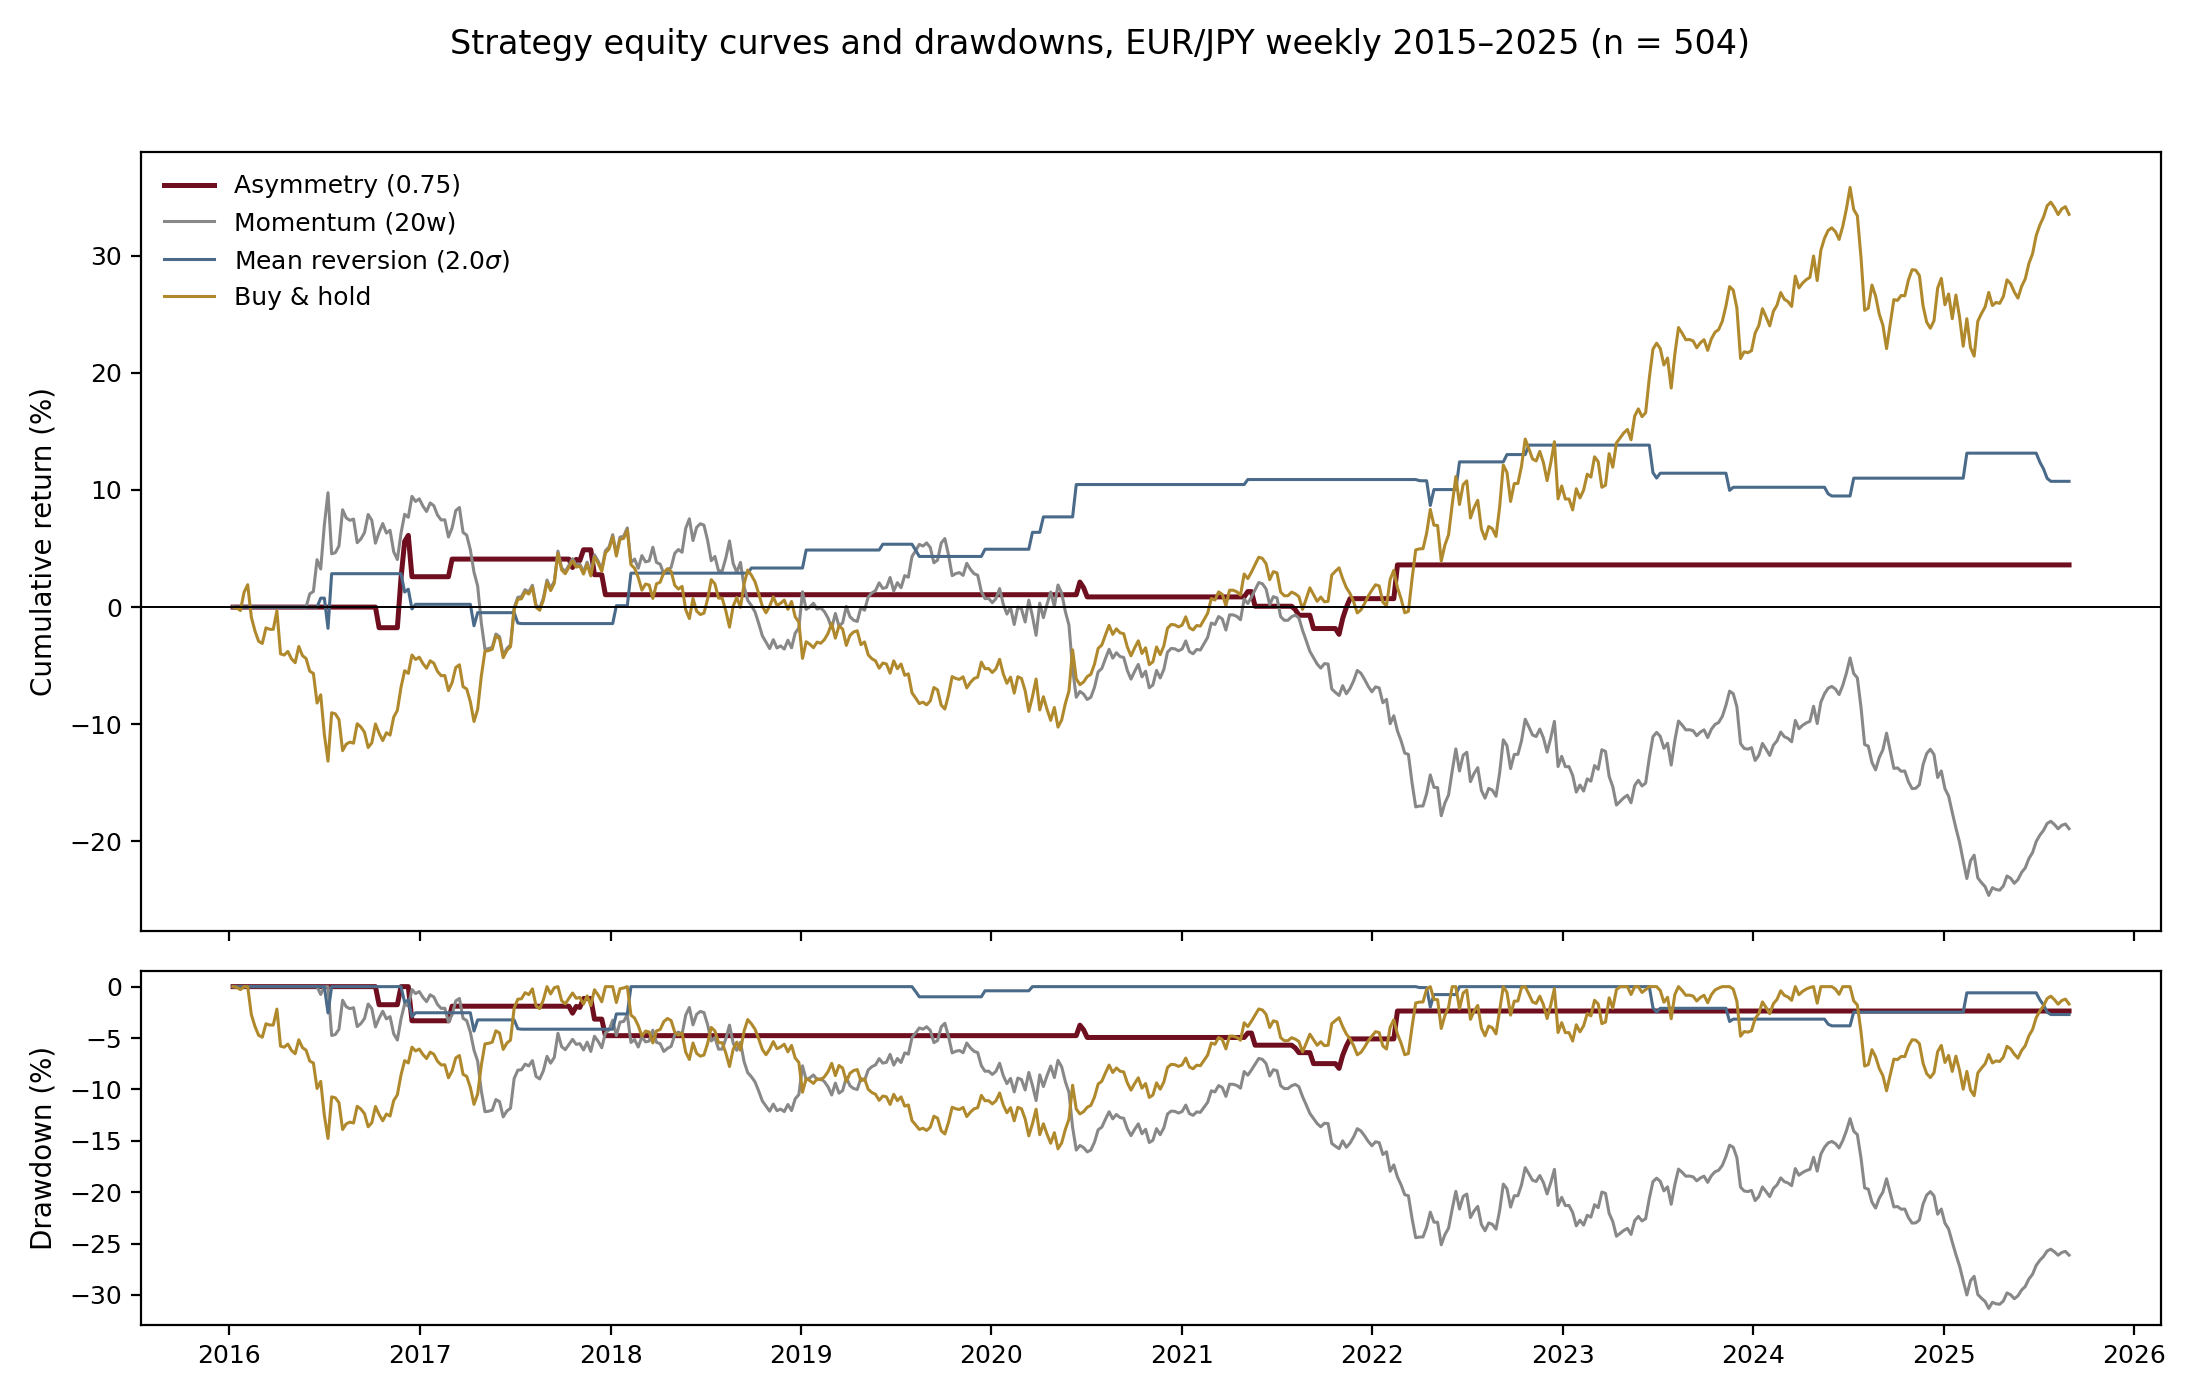
\includegraphics[width=\textwidth]{backtest_results.png}
\caption{Strategy equity curves and drawdowns (enlarged). Cumulative gross returns and drawdown profiles for the asymmetry strategy, the 20-week momentum and 2.0$\sigma$ mean-reversion benchmarks, and buy-and-hold on the 504-week EUR/JPY sample.}
\label{fig:backtest-enlarged}
\end{figure}

\end{document}
